\section{Graph Theory and Spectral Analysis}

The attention mechanisms developed so far operate on data with regular structure (sequences, images, point clouds). However, many problems of interest (social networks, molecules, knowledge graphs) involve data with irregular connectivity. The natural extension of attention to these domains requires combining graph theory with spectral analysis, providing solid mathematical foundations for adaptive weights on irregularly structured data.

\subsection{Graph Foundations}

For the graph theory foundations (definition of a graph, adjacency matrix, Laplacian) needed in attention mechanisms, see \autoref{ch:gdl}, \autoref{sec:grafos_discretizacion}. The spectral analysis concepts are developed in \autoref{ch:cnn}.

\subsubsection{Connection with Message Passing}

Attention mechanisms on graphs generalize the message passing paradigm:

\begin{equation}
    \text{Attention} \equiv \text{MessagePassing with adaptive weights}
    \label{eq:attention_message_passing_equivalence}
\end{equation}

\subsection{Graph Attention Networks}\label{subsec:graph_attention_networks}\label{sec:graph_attention}

\glspl{GAT} represent the natural intersection between the spectral theory of graphs developed in \autoref{sec:analisis_armonico} and adaptive attention mechanisms. While traditional spectral methods require expensive eigendecomposition, \glspl{GAT} achieve similar expressive power through learnable attention coefficients that implicitly capture the structure of the graph and long-range dependencies.

\subsubsection{Mathematical Foundations: Attention over Graphs}\label{subsubsec:fundamentos_atencion_grafos}

\begin{definition}[Labeled Graph for Attention]\label{def:labeled_graph_attention}
A \textit{labeled graph for attention} is a tuple $\mathcal{G} = (V, E, \mathbf{H})$ where:
\begin{itemize}
    \item $V = \{v_1, v_2, \ldots, v_n\}$ is the set of nodes
    \item $E \subseteq V \times V$ is the set of edges
    \item $\mathbf{H} = [\mathbf{h}_1, \mathbf{h}_2, \ldots, \mathbf{h}_n]^T \in \mathbb{R}^{n \times d}$ are the node features
\end{itemize}
The structure of the graph defines the attention constraints: typically, node $v_i$ can attend only to its neighborhood $\mathcal{N}(i) = \{j : (i,j) \in E\}$.
\end{definition}

\begin{definition}[Graph Attention Function]\label{def:graph_attention_function}
A \textit{graph attention function} $f_{\text{GAT}}: \mathcal{G} \to \mathbb{R}^{n \times d'}$ satisfies:
\begin{enumerate}
    \item \textbf{Permutation equivariance}: For any permutation $\pi$ of the nodes:
    \begin{equation}
        f_{\text{GAT}}(\pi(\mathcal{G})) = \pi(f_{\text{GAT}}(\mathcal{G}))
        \label{eq:gat_permutation_equivariance}
    \end{equation}

    \item \textbf{Respect for structure}: It only considers connections defined by $E$:
    \begin{equation}
        \frac{\partial f_{\text{GAT}}(\mathbf{h}_i)}{\partial \mathbf{h}_j} \neq \mathbf{0} \Rightarrow (i,j) \in E \text{ or } i = j
        \label{eq:gat_structural_constraint}
    \end{equation}
\end{enumerate}
\end{definition}

\subsubsection{Classical Graph Attention Networks}\label{subsubsec:gat_clasicos}

The pioneering work of \citet{velickovic2017graph} introduces the first successful formulation of attention specific to graphs.

\begin{definition}[GAT Attention Mechanism]\label{def:gat_mechanism}
For a node $i$ with neighborhood $\mathcal{N}(i)$, the \gls{GAT} mechanism computes:

\textbf{Step 1: Linear projection}
\begin{equation}
    \mathbf{z}_i = \mathbf{W}\mathbf{h}_i, \quad \mathbf{z}_j = \mathbf{W}\mathbf{h}_j
    \label{eq:gat_linear_projection}
\end{equation}
where $\mathbf{W} \in \mathbb{R}^{d' \times d}$ is a shared weight matrix.

\textbf{Step 2: Attention coefficients}
\begin{equation}
    e_{ij} = a^T[\mathbf{z}_i \| \mathbf{z}_j] = a^T[\mathbf{W}\mathbf{h}_i \| \mathbf{W}\mathbf{h}_j]
    \label{eq:gat_attention_coefficients}
\end{equation}
where $a \in \mathbb{R}^{2d'}$ is a learnable attention vector and $\|$ denotes concatenation.

\textbf{Step 3: Masked softmax normalization}
\begin{equation}
    \alpha_{ij} = \frac{\exp(\text{LeakyReLU}(e_{ij}))}{\sum_{k \in \mathcal{N}(i) \cup \{i\}} \exp(\text{LeakyReLU}(e_{ik}))}
    \label{eq:gat_softmax_normalization}
\end{equation}

\textbf{Step 4: Weighted aggregation}
\begin{equation}
    \mathbf{h}_i' = \sigma\left(\sum_{j \in \mathcal{N}(i) \cup \{i\}} \alpha_{ij} \mathbf{z}_j\right)
    \label{eq:gat_weighted_aggregation}
\end{equation}
\end{definition}

\begin{figure}[ht]
\centering
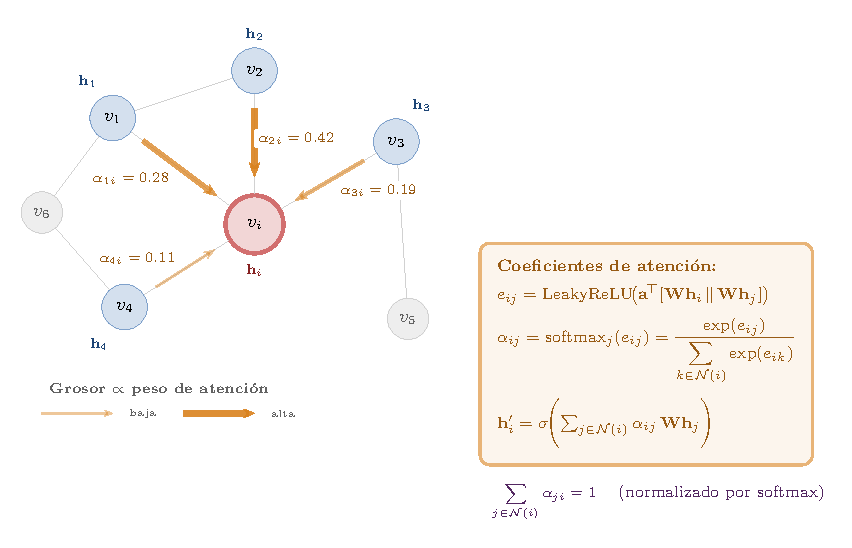
\includegraphics[width=0.75\textwidth]{images/gat_mechanism.pdf}
\caption{Graph Attention Network (GAT) mechanism. The central node (red) computes attention coefficients $\alpha_{ij}$ with each neighbor (blue). The thickness of the arrows reflects the magnitude of the attention weights: the network learns to assign different importances to each neighbor according to the node features.}
\label{fig:gat_mechanism}
\end{figure}

\begin{proposition}[Expressive Power of GAT]\label{prop:gat_expressive_power}
Standard Graph Attention Networks are bounded in expressive power by the 1-Weisfeiler-Lehman (1-WL) test \citep{xu2019how}. This implies:
\begin{enumerate}
    \item \textbf{Upper bound}: GAT cannot distinguish pairs of non-isomorphic graphs that the 1-WL test does not distinguish.
    \item \textbf{Anisotropic aggregation}: Unlike \gls{GCN} with fixed weights, GAT can learn adaptive aggregation functions through attention coefficients, which allows greater flexibility within the class of functions accessible by message passing architectures.
    \item \textbf{Permutation equivariance}: GAT is permutation-equivariant by construction, since the attention coefficients depend only on the features of the nodes involved and not on an ordering.
\end{enumerate}
\end{proposition}

\begin{proof}
GAT is an instance of the MPNN (message passing neural network) framework with attention-weighted aggregation over the 1-hop neighborhood. \citet{xu2019how} prove that every MPNN architecture is bounded by the 1-WL test in its capacity to distinguish graphs. Permutation equivariance follows from the fact that the attention operation is invariant to the reordering of neighboring nodes: the coefficients $\alpha_{ij}$ depend on $(\mathbf{h}_i, \mathbf{h}_j)$ and the aggregation $\sum_{j \in \mathcal{N}(i)} \alpha_{ij} \mathbf{z}_j$ is symmetric with respect to the order of the neighbors.
\end{proof}

\subsubsection{Multi-Head Graph Attention}\label{subsubsec:multihead_graph_attention}

To improve stability and expressive capacity, \glspl{GAT} employ multi-head attention.

\begin{definition}[Multi-Head GAT]\label{def:multihead_gat}
A Multi-Head GAT with $h$ heads computes:

\begin{equation}
    \mathbf{h}_i' = \sigma\left(\frac{1}{h}\sum_{k=1}^{h} \sum_{j \in \mathcal{N}(i)} \alpha_{ij}^{(k)} \mathbf{W}^{(k)}\mathbf{h}_j\right)
    \label{eq:multihead_gat_average}
\end{equation}

or through concatenation:

\begin{equation}
    \mathbf{h}_i' = \sigma\left(\|_{k=1}^{h} \sum_{j \in \mathcal{N}(i)} \alpha_{ij}^{(k)} \mathbf{W}^{(k)}\mathbf{h}_j\right)
    \label{eq:multihead_gat_concat}
\end{equation}

where each head $k$ has its own parameters $\mathbf{W}^{(k)}$ and $\mathbf{a}^{(k)}$.
\end{definition}

\begin{proposition}[Advantages of Multi-Head GAT]\label{prop:multihead_gat_advantages}
The Multi-Head GAT provides:
\begin{enumerate}
    \item \textbf{Training stability}: Reduces the variance of the gradients
    \item \textbf{Feature specialization}: Different heads capture different relational aspects
    \item \textbf{Greater expressive capacity}: Approximates more complex functions with the same total number of parameters
\end{enumerate}
\end{proposition}

\begin{proof}[Justification]
\textbf{(1)} Let $\hat{\mathbf{h}}_i^{(k)} = \frac{1}{H}\sum_{h=1}^H \mathbf{h}_i^{(k,h)}$ be the averaged output. The variance of the gradient $\text{Var}[\nabla_\theta \hat{\mathbf{h}}_i]$ is reduced by a factor $1/H$ relative to a single head, due to the independence of the attention mechanisms in each head (analogous to the effect of \textit{ensemble methods}).

\textbf{(2)} Empirically, the heads tend to specialize: with $H$ heads and dimension $d/H$ each, every head operates in a different subspace of $\mathbb{R}^d$. The attention weights $\alpha_{ij}^{(h)}$ vary significantly across heads, indicating that they capture different relational patterns.

\textbf{(3)} The space of functions representable by $H$ heads of dimension $d/H$ strictly includes that of a single head of dimension $d$: the concatenation $\|_{h=1}^H \text{Attn}_h$ can represent functions that require attending simultaneously to distinct combinations of neighbors, which a single head cannot achieve.
\end{proof}

\subsubsection{Spectral Analysis of Graph Attention}\label{subsubsec:analisis_espectral_gat}

The connection between GATs and spectral analysis reveals deep insights into how they work.

\begin{definition}[Spectral Interpretation of Attention]\label{def:spectral_interpretation_attention}
Let $\mathbf{A}^{(GAT)} \in \mathbb{R}^{n \times n}$ be the attention matrix with entries $A^{(GAT)}_{ij} = \alpha_{ij}$. This matrix can be interpreted as a \textbf{learnable version of the diffusion operator}:
\begin{equation}
    \mathbf{A}^{(GAT)} \approx f(\mathbf{L}^{-1})
    \label{eq:gat_spectral_approximation}
\end{equation}
where $f$ is a learnable function and $\mathbf{L}$ is the \gls{laplaciano_grafo}.
\end{definition}

\begin{theorem}[GAT-Spectral Connection]\label{thm:gat_spectral_connection}
In the limit of many layers, a \gls{GAT} with stable attention weights converges to performing adaptive spectral filtering:
\begin{equation}
    \lim_{L \to \infty} \text{GAT}^{(L)}(\mathbf{H}) = \mathbf{U} \text{diag}(\hat{g}(\lambda_1), \ldots, \hat{g}(\lambda_n)) \mathbf{U}^T \mathbf{H}
    \label{eq:gat_spectral_limit}
\end{equation}
where $\mathbf{U}$ contains the eigenvectors of the Laplacian and $\hat{g}$ is the implicitly learned filter function.
\end{theorem}

\begin{proof}
\textbf{Step 1}: Stability of the attention weights.
In the limit, the attention weights converge: $\lim_{L \to \infty} \alpha_{ij}^{(L)} = \alpha_{ij}^*$.

\textbf{Step 2}: Limiting transition matrix.
The \gls{GAT} operation becomes: $\mathbf{H}^{(L+1)} = \mathbf{A}^* \mathbf{H}^{(L)}$ where $\mathbf{A}^*$ is the stable attention matrix.

\textbf{Step 3}: Spectral decomposition.
Under the (idealized) hypothesis that $\mathbf{A}^*$ shares eigenvectors with the Laplacian of the graph: $\mathbf{A}^* = \mathbf{U} \mathbf{\Lambda}^* \mathbf{U}^T$.

\textbf{Step 4}: Implicit filtering.
The eigenvalues $\mathbf{\Lambda}^*$ implicitly define the filter function $\hat{g}$.
\end{proof}

\begin{remark}
Step~3 of the previous proof assumes that the learned attention matrix $\mathbf{A}^*$ shares eigenvectors with the Laplacian of the graph $\mathbf{L}$, which is a simplification. In practice, $\mathbf{A}^*$ is generally asymmetric and its eigenvectors do not coincide with those of $\mathbf{L}$. This spectral connection should be understood as an analogy that holds exactly only when the attention coefficients are functions of the graph structure compatible with its spectral decomposition. Moreover, the repeated application of a fixed stochastic matrix $\mathbf{A}^*$ converges to a stationary distribution (the over-smoothing phenomenon), not to the rich spectral filtering described in equation~\eqref{eq:gat_spectral_limit}.
\end{remark}

\subsubsection{Spectral Positional Encoding}\label{subsubsec:codificacion_posicional_espectral}

A fundamental limitation of \glspl{GAT} is their inability to distinguish structurally equivalent nodes. Spectral positional encoding solves this problem.

\begin{definition}[Spectral Positional Encoding]\label{def:spectral_positional_encoding}
Let $\mathbf{L} = \mathbf{U}\mathbf{\Lambda}\mathbf{U}^T$ be the spectral decomposition of the \gls{laplaciano_grafo}. The spectral positional encoding of node $i$ is defined as:
\begin{equation}
    \text{PE}_i = [\mathbf{u}_{i,1}, \mathbf{u}_{i,2}, \ldots, \mathbf{u}_{i,k}] \in \mathbb{R}^k
    \label{eq:spectral_positional_encoding}
\end{equation}
where $\mathbf{u}_{i,j}$ is the $i$-th component of the $j$-th smallest eigenvector (excluding the trivial one).
\end{definition}

\begin{definition}[Spectral Distances for Attention]\label{def:spectral_distances_attention}
To improve attention between distant nodes, spectral metrics are defined:

\textbf{Diffusion Distance}:
\begin{equation}
    d_D^2(i,j) = \sum_{k=2}^{n} e^{-2t\lambda_k} (\mathbf{u}_{i,k} - \mathbf{u}_{j,k})^2
    \label{eq:diffusion_distance}
\end{equation}

\textbf{Green's Function}:
\begin{equation}
    G(i,j) = \sum_{k=2}^{n} \frac{\mathbf{u}_{i,k} \mathbf{u}_{j,k}}{\lambda_k}
    \label{eq:green_function_distance}
\end{equation}

\textbf{Biharmonic Distance}:
\begin{equation}
    d_B^2(i,j) = \sum_{k=2}^{n} \frac{(\mathbf{u}_{i,k} - \mathbf{u}_{j,k})^2}{\lambda_k^2}
    \label{eq:biharmonic_distance}
\end{equation}
\end{definition}

\subsubsection{Spectral Attention Networks (SAN)}\label{subsubsec:spectral_attention_networks}

\citet{kreuzer2021spectral} introduce the first fully connected Transformer for graphs that competes with specialized GNNs.

\begin{definition}[SAN Architecture]\label{def:san_architecture}
A Spectral Attention Network processes graphs through:

\textbf{Step 1: Learnable positional encoding}
\begin{equation}
    \text{LPE}_i = \text{MLP}_{\text{PE}}([\lambda_1, \ldots, \lambda_k, \mathbf{u}_{i,1}, \ldots, \mathbf{u}_{i,k}])
    \label{eq:learned_positional_encoding}
\end{equation}

\textbf{Step 2}: Dual attention (real + virtual)
\begin{align}
    \mathbf{h}_i^{\text{real}} &= \text{Attention}_{\text{sparse}}(\mathbf{h}_i, \{\mathbf{h}_j : j \in \mathcal{N}(i)\}) \\
    \mathbf{h}_i^{\text{virtual}} &= \text{Attention}_{\text{full}}(\mathbf{h}_i, \{\mathbf{h}_j : j \in V\})
    \label{eq:dual_attention_san}
\end{align}

\textbf{Step 3: Adaptive balancing}
\begin{equation}
    \mathbf{h}_i' = \gamma \cdot \mathbf{h}_i^{\text{real}} + (1-\gamma) \cdot \mathbf{h}_i^{\text{virtual}}
    \label{eq:adaptive_balancing_san}
\end{equation}
where $\gamma \in [0,1]$ is a learnable parameter.
\end{definition}

\begin{theorem}[Overcoming Over-Squashing]\label{thm:over_squashing_resolution}
Spectral Attention Networks solve the over-squashing problem by providing direct connections between arbitrarily distant nodes:
\begin{equation}
    \text{Information distance} = \mathcal{O}(1) \quad \forall i,j \in V
    \label{eq:information_distance_constant}
\end{equation}
independently of the geodesic distance in the original graph.
\end{theorem}

\begin{proof}
In a \gls{GNN} with local message passing, the information of node $j$ takes at least $d_G(i,j)$ layers to reach node $i$, where $d_G$ is the geodesic distance. After $L$ layers, the information is compressed into fixed-dimension representations $d$, causing over-squashing when $|\{j: d_G(i,j) \leq L\}|$ grows exponentially \citep{topping2022understanding}. In SAN, global attention allows node $i$ to attend directly to node $j$ in a single layer, with score $\alpha_{ij} = \text{softmax}(\mathbf{q}_i^T \mathbf{k}_j / \sqrt{d})$. The information distance $D_{\text{info}}(i,j) = -\log \alpha_{ij}$ is $O(1)$ (it depends on the similarity of representations, not on the topology of the graph), eliminating the bottleneck.
\end{proof}

\subsubsection{Scalable Extensions: GraphGPS}\label{subsubsec:graphgps}

\begin{definition}[GraphGPS Architecture]\label{def:graphgps_architecture}
GraphGPS \citep{rampasek2022graphgps} combines local message passing with global attention through:

\begin{equation}
    \mathbf{H}^{(\ell+1)} = \text{MLP}^{(\ell)}\left(\mathbf{H}_{\text{MPNN}}^{(\ell+1)} + \mathbf{H}_{\text{Global}}^{(\ell+1)}\right)
    \label{eq:graphgps_architecture}
\end{equation}

where:
\begin{align}
    \mathbf{H}_{\text{MPNN}}^{(\ell+1)} &= \text{MPNN}^{(\ell)}(\mathbf{H}^{(\ell)}) \\
    \mathbf{H}_{\text{Global}}^{(\ell+1)} &= \text{GlobalTransformer}^{(\ell)}(\mathbf{H}^{(\ell)} + \text{PE})
    \label{eq:graphgps_components}
\end{align}
\end{definition}

\begin{proposition}[Linear Scalability of GraphGPS]\label{prop:graphgps_scalability}
When a linear-complexity attention mechanism (Performer \citep{choromanski2021performer} or BigBird) is used for the global component, and excluding the cost of precomputing spectral positional encodings, GraphGPS achieves per-layer complexity $\mathcal{O}(N + E)$ through:
\begin{enumerate}
    \item \textbf{Sub-quadratic attention}: Performer or BigBird with complexity $\mathcal{O}(N)$
    \item \textbf{Local message passing}: Complexity $\mathcal{O}(E)$ for the MPNN component
    \item \textbf{Modular separation}: Decoupling of local and global information
\end{enumerate}
With standard full attention, the global component would have complexity $\mathcal{O}(N^2)$. For the precise breakdown as a function of the model parameters, see \autoref{prop:graphgps_efficient_complexity}.
\end{proposition}

\begin{proof}
The complexity is obtained by summing the contributions of each component. The MPNN component processes each edge once, resulting in $\mathcal{O}(E)$. For the global component, mechanisms like Performer approximate softmax attention through $\text{softmax}(\mathbf{Q}\mathbf{K}^\top) \approx \hat{\phi}(\mathbf{Q})\hat{\phi}(\mathbf{K})^\top$, where $\hat{\phi}: \mathbb{R}^d \to \mathbb{R}^k$ with $k \ll N$. This reduces the computation from $\mathcal{O}(N^2)$ to $\mathcal{O}(Nk) = \mathcal{O}(N)$ for fixed $k$. The modular separation allows summing both contributions independently, obtaining $\mathcal{O}(N + E)$.
\end{proof}

\subsubsection{Limitations and Future Directions}\label{subsubsec:limitaciones_gat}

\paragraph{Current Limitations}

\begin{enumerate}
    \item \textbf{1-WL limitation}: Standard GATs cannot distinguish non-isomorphic graphs that the 1-Weisfeiler-Lehman test cannot distinguish

    \item \textbf{Over-smoothing}: In deep graphs, the node representations converge to similar values:
    \begin{equation}
        \lim_{L \to \infty} \|\mathbf{h}_i^{(L)} - \mathbf{h}_j^{(L)}\| \to 0 \quad \forall i,j
        \label{eq:over_smoothing_limit}
    \end{equation}

    \item \textbf{Sign ambiguity}: The eigenvectors are defined up to multiplication by $\pm 1$, requiring techniques such as SignNet

    \item \textbf{Isospectral graphs}: Graphs with identical spectra but different structures cannot be distinguished spectrally
\end{enumerate}

\paragraph{Future Research}

\begin{definition}[Higher-Order k-GAT]\label{def:higher_order_gat}
Higher-order GATs consider $k$-tuples of nodes:
\begin{equation}
    \alpha_{i,\mathcal{S}} = \text{softmax}\left(a^T\left[\|_{j \in \mathcal{S}} \mathbf{W}\mathbf{h}_j\right]\right)
    \label{eq:higher_order_gat}
\end{equation}
where $\mathcal{S} \subseteq \mathcal{N}^{(k)}(i)$ is a $k$-subset of the $k$-neighborhood.
\end{definition}

\begin{definition}[Continuous Geometric Attention]\label{def:continuous_geometric_attention}
For graphs embedded in continuous spaces:
\begin{equation}
    e_{ij} = a(\mathbf{h}_i, \mathbf{h}_j, \|\mathbf{x}_i - \mathbf{x}_j\|, \angle(\mathbf{x}_i, \mathbf{x}_j))
    \label{eq:continuous_geometric_attention}
\end{equation}
incorporating metric and angular information.
\end{definition}

\subsubsection{Connections with Previous Chapters}

The developments in GATs connect directly with established concepts:

\begin{itemize}
    \item \textbf{Spectral Analysis (\autoref{sec:analisis_armonico})}: GATs implicitly implement adaptive spectral filtering
    \item \textbf{Message Passing (Section~\ref{subsec:message_passing_unificador})}: GATs are a specific instantiation of the unifying framework with attention-based aggregation
    \item \textbf{Equivariance (Section~\ref{subsec:equivarianza_invarianza})}: GATs preserve permutation equivariance while gaining adaptive flexibility
\end{itemize}

\begin{proposition}[Synthesis of GAT in the Unifying Framework]\label{prop:gat_unified_framework}
Graph Attention Networks are naturally expressed in the Geometric Message Passing framework:
\begin{align}
    \mathbf{h}_i^{(k+1)} &= \phi^{(k)}\left(\mathbf{h}_i^{(k)}, \bigoplus_{j \in \mathcal{N}(i)} \alpha_{ij} \cdot \psi^{(k)}(\mathbf{h}_j^{(k)})\right) \\
    \alpha_{ij} &= \text{Attention}(\mathbf{h}_i^{(k)}, \mathbf{h}_j^{(k)}, e_{ij})
    \label{eq:gat_in_unified_framework}
\end{align}
where the attention weights $\alpha_{ij}$ replace the fixed aggregation with learnable adaptive aggregation.
\end{proposition}

\begin{proof}
Let $G = (V, E)$ be a graph and $\mathbf{h}_i^{(k)}$ the representation of node $i$ in layer $k$. In the standard MPNN framework, the update takes the form $\mathbf{h}_i^{(k+1)} = \phi(\mathbf{h}_i^{(k)}, \bigoplus_{j \in \mathcal{N}(i)} \psi(\mathbf{h}_j^{(k)}))$. In a GAT, the message function is $\psi^{(k)}(\mathbf{h}_j) = \mathbf{W}^{(k)} \mathbf{h}_j$ and the aggregation is $\bigoplus = \sum_{j} \alpha_{ij} (\cdot)$, where $\alpha_{ij} = \operatorname{softmax}_j(e_{ij})$ with $e_{ij} = \text{LeakyReLU}(\mathbf{a}^\top [\mathbf{W}\mathbf{h}_i \| \mathbf{W}\mathbf{h}_j])$. Substituting into the general MPNN equation directly yields the expression in the proposition.
\end{proof}

This formulation shows that GATs represent the natural evolution of message passing from rigid aggregation toward flexible aggregation, maintaining equivariance guarantees while gaining adaptive expressiveness.

\subsection{Spectral Analysis on Graphs}

For the spectral analysis foundations of the Laplacian, including eigenvalues, eigenvectors, and spectral decomposition, see \autoref{ch:cnn}, Detailed Spectral Analysis Section. The spectral positional encoding (\autoref{def:spectral_positional_encoding}) and the spectral distances (\autoref{def:spectral_distances_attention}) introduced earlier constitute the fundamental tools for incorporating structural information of the graph into attention mechanisms.

\subsection{Advanced Graph Architectures}\label{subsec:arquitecturas_avanzadas_grafos}

Advanced graph architectures represent the confluence of attention mechanisms with the fundamental principles of \gls{GDL} developed in \autoref{ch:gdl}. This section examines how different architectural designs integrate spectral, structural, and geometric information to overcome the limitations of basic architectures such as GAT. Each architecture addresses specific challenges: Spectral Attention Networks solve the problem of positional ambiguity, GraphGPS combines local and global processing efficiently, Graph \glspl{Transformer} incorporate topological structure into attention, and Structure-Aware \glspl{Transformer} exploit subgraph patterns. We will unify these architectures by showing how they instantiate the Message Passing framework (Section~\ref{subsec:message_passing_unificador}) with different aggregation mechanisms and inductive biases.

\subsubsection{Spectral Attention Networks}\label{subsubsec:san_advanced}

The Spectral Attention Networks of \citet{kreuzer2021spectral} constitute the first fully connected \gls{Transformer} for graphs that competes with specialized \glspl{GNN}. Their fundamental contribution lies in the use of learnable positional encodings based on the spectrum of the graph Laplacian.

\paragraph{Theoretical foundation: the isotropy problem}

Standard \glspl{Transformer} operate on sequences with an implicit natural order, which provides intrinsic positional information. Graphs, however, lack a canonical ordering: they are invariant under node permutations. This invariance, although desirable from the perspective of equivariance (see Section~\ref{subsec:equivarianza_invarianza}), eliminates all structural positional information. The central challenge is: \textit{how can a \gls{Transformer} be endowed with positional information in a domain without a natural order?}

SAN's answer is to use the \textbf{spectrum of the graph Laplacian}. The Spectral Theorem (\autoref{ch:cnn}) guarantees that for the symmetric normalized Laplacian $\tilde{L} = I - D^{-1/2}AD^{-1/2}$ there exists a decomposition:
\begin{equation}
    \tilde{L} = \sum_{k=1}^{n} \lambda_k \mathbf{v}_k \mathbf{v}_k^T
    \label{eq:spectral_decomposition_san}
\end{equation}
where $0 = \lambda_1 \leq \lambda_2 \leq \cdots \leq \lambda_n \leq 2$ are the eigenvalues and $\{\mathbf{v}_k\}_{k=1}^{n}$ the corresponding orthonormal eigenvectors.

\begin{definition}[Learnable Spectral Positional Encoding]\label{def:learned_spectral_pe}
For a graph $G$ with Laplacian $\tilde{L}$, the learnable spectral positional encoding for node $i$ is defined as:
\begin{equation}
    \mathbf{PE}_i = \text{MLP}_{\text{enc}}(\lambda_1, \ldots, \lambda_k, \mathbf{v}_{1,i}, \ldots, \mathbf{v}_{k,i}) \in \mathbb{R}^{d_{\text{model}}}
    \label{eq:san_learned_positional_encoding}
\end{equation}
where:
\begin{itemize}
    \item $k \ll n$ is the number of spectral components used (typically $k \in [8, 20]$)
    \item $\text{MLP}_{\text{enc}}$ is a multilayer network with a nonlinear activation function
    \item $\lambda_1, \ldots, \lambda_k$ are the first $k$ eigenvalues (global information of the graph)
    \item $\mathbf{v}_{k,i}$ is the $i$-th component of the eigenvector $\mathbf{v}_k$ (local positional information of the node)
\end{itemize}
\end{definition}

\textbf{Spectral justification.}\label{rem:justification_spectral_pe} The first eigenvectors of the Laplacian capture fundamental topological structure:
\begin{itemize}
    \item $\mathbf{v}_1 = \frac{1}{\sqrt{n}}\mathbf{1}$ (constant vector, connected component)
    \item $\mathbf{v}_2$ (Fiedler vector) identifies communities and minimum cuts
    \item Subsequent eigenvectors capture geometric patterns of increasing frequency
\end{itemize}
This approach connects with harmonic analysis on graphs (\autoref{ch:cnn}), where the eigenvectors form a Fourier basis for signals over the graph.

\paragraph{SAN architecture: dual attention with adaptive balancing}

The complete SAN architecture implements a \textbf{dual attention} scheme that combines local information (graph neighborhood) with global information (the full graph):

\begin{definition}[SAN Layer]\label{def:san_layer}
A SAN layer processes node features $\mathbf{H}^{(\ell)} \in \mathbb{R}^{n \times d}$ through three stages:

\textbf{Stage 1: Positional encoding injection}
\begin{equation}
    \tilde{\mathbf{H}}^{(\ell)} = \mathbf{H}^{(\ell)} + \mathbf{PE}
    \label{eq:san_pe_injection}
\end{equation}

\textbf{Stage 2: Dual attention}
\begin{align}
    \mathbf{H}_{\text{local}}^{(\ell+1)} &= \text{MultiHeadAttn}_{\text{sparse}}\left(\tilde{\mathbf{H}}^{(\ell)}, \mathcal{E}\right) \label{eq:san_local_attn} \\
    \mathbf{H}_{\text{global}}^{(\ell+1)} &= \text{MultiHeadAttn}_{\text{full}}\left(\tilde{\mathbf{H}}^{(\ell)}\right) \label{eq:san_global_attn}
\end{align}
where $\mathcal{E}$ denotes the edges of the graph and the sparse attention only computes weights for pairs $(i,j) \in \mathcal{E}$.

\textbf{Stage 3: Adaptive combination}
\begin{equation}
    \mathbf{H}^{(\ell+1)} = \text{MLP}\left(\text{LayerNorm}\left(\gamma^{(\ell)} \mathbf{H}_{\text{local}}^{(\ell+1)} + (1-\gamma^{(\ell)}) \mathbf{H}_{\text{global}}^{(\ell+1)}\right)\right)
    \label{eq:san_adaptive_combination}
\end{equation}
where $\gamma^{(\ell)} \in [0,1]$ is a learnable parameter per layer.
\end{definition}

\begin{proposition}[Computational Complexity of SAN]\label{prop:san_complexity}
A SAN layer with $n$ nodes, $m$ edges, $h$ attention heads, and dimension $d$ has complexity:
\begin{equation}
    \mathcal{O}(hd(m + n^2)) = \mathcal{O}(hdm) + \mathcal{O}(hdn^2)
    \label{eq:san_complexity}
\end{equation}
The quadratic term $\mathcal{O}(hdn^2)$ dominates for dense graphs, limiting scalability to graphs with thousands of nodes.
\end{proposition}

\begin{proof}
Local attention operates over the $m$ edges of the graph: for each edge $(i,j)$, each head computes attention scores and messages in $\mathcal{O}(d)$, giving $\mathcal{O}(hdm)$. Global attention computes the matrix $\mathbf{Q}\mathbf{K}^\top \in \mathbb{R}^{n \times n}$ for each head, requiring $\mathcal{O}(dn^2)$ operations per head and $\mathcal{O}(hdn^2)$ in total. The subsequent multiplication with $\mathbf{V}$ is also $\mathcal{O}(hdn^2)$. Summing both contributions gives $\mathcal{O}(hd(m + n^2))$.
\end{proof}

\subsubsection{GraphGPS: Modular and Scalable Design}\label{subsubsec:graphgps_advanced}

GraphGPS (Graph Generalized Positional Signals) by \citet{rampasek2022graphgps} represents an evolution toward modular and composable architectures. Its design philosophy is based on three principles:

\begin{enumerate}
    \item \textbf{Separation of responsibilities}: Specialized components for local vs. global processing
    \item \textbf{Scalability}: Use of efficient attention mechanisms (Performer, BigBird)
    \item \textbf{Flexibility}: Interchangeability of MPNN and attention components
\end{enumerate}

\paragraph{Modular architecture}

\begin{definition}[GraphGPS Layer]\label{def:graphgps_layer}
A GraphGPS layer consists of two parallel paths that are merged:
\begin{equation}
    \mathbf{H}^{(\ell+1)} = \mathbf{H}^{(\ell)} + \text{MLP}^{(\ell)}\left(\text{LayerNorm}\left(\mathbf{H}_{\text{MPNN}}^{(\ell)} + \mathbf{H}_{\text{Global}}^{(\ell)}\right)\right)
    \label{eq:graphgps_main_layer}
\end{equation}

\textbf{Local path (Message Passing):}
\begin{equation}
    \mathbf{H}_{\text{MPNN}}^{(\ell)} = \text{MPNN}^{(\ell)}\left(\mathbf{H}^{(\ell)}, \mathcal{E}\right)
    \label{eq:graphgps_mpnn_path}
\end{equation}
where $\text{MPNN}^{(\ell)}$ can be \gls{GCN}, \gls{GAT}, GIN, or any message passing architecture.

\textbf{Global path (Attention with PE):}
\begin{equation}
    \mathbf{H}_{\text{Global}}^{(\ell)} = \text{Transformer}^{(\ell)}\left(\mathbf{H}^{(\ell)} + \mathbf{PE}\right)
    \label{eq:graphgps_global_path}
\end{equation}
where the \gls{Transformer} can use full attention, Performer, or BigBird for efficiency.
\end{definition}

\textbf{Interpretation as a sum of aggregations.}\label{rem:graphgps_interpretation} GraphGPS implements an additive decomposition of aggregation in the Message Passing framework (Section~\ref{subsec:message_passing_unificador}):
\begin{equation}
    m_i^{(\ell)} = \underbrace{\bigoplus_{j \in \mathcal{N}(i)} \psi_{\text{local}}(\mathbf{h}_j^{(\ell)})}_{\text{Local aggregation (MPNN)}} + \underbrace{\bigoplus_{j \in V} \alpha_{ij}^{(\ell)} \psi_{\text{global}}(\mathbf{h}_j^{(\ell)})}_{\text{Global aggregation (Attention)}}
    \label{eq:graphgps_message_decomposition}
\end{equation}
This decomposition allows capturing both local patterns (topological structure) and long-range dependencies (global interactions).

\paragraph{Scalability mechanisms}

\begin{proposition}[Complexity of GraphGPS with efficient attention]\label{prop:graphgps_efficient_complexity}
Using Performer for global attention, GraphGPS achieves complexity:
\begin{equation}
    \mathcal{O}(hdm + ndk) \quad \text{where } k \ll n
    \label{eq:graphgps_linear_complexity}
\end{equation}
with $k$ the rank of the Performer approximation. For graphs with $m = \mathcal{O}(n)$, the total complexity is $\mathcal{O}(ndk)$, linear in the number of nodes.
\end{proposition}

\begin{proof}
The MPNN component processes the $m$ edges with $h$ heads of dimension $d$, contributing $\mathcal{O}(hdm)$. For the global component, Performer replaces the explicit computation of $\mathbf{Q}\mathbf{K}^\top \in \mathbb{R}^{n \times n}$ with the approximation $\hat{\phi}(\mathbf{Q})(\hat{\phi}(\mathbf{K})^\top \mathbf{V})$, where $\hat{\phi}: \mathbb{R}^d \to \mathbb{R}^k$. The product $\hat{\phi}(\mathbf{K})^\top \mathbf{V} \in \mathbb{R}^{k \times d}$ is computed in $\mathcal{O}(ndk)$ and then $\hat{\phi}(\mathbf{Q}) \cdot (\hat{\phi}(\mathbf{K})^\top \mathbf{V})$ also in $\mathcal{O}(ndk)$. Summing: $\mathcal{O}(hdm + ndk)$. If $m = \mathcal{O}(n)$ and $h, k$ are constant with respect to $n$, this reduces to $\mathcal{O}(ndk)$.
\end{proof}

\begin{example}[Typical GraphGPS configuration]\label{ex:graphgps_configuration}
A standard configuration uses:
\begin{itemize}
    \item \textbf{Local MPNN}: GatedGCN (8 layers)
    \item \textbf{Global attention}: Performer with $k=256$ random features
    \item \textbf{Positional encoding}: Laplacian eigenvectors (10 components) + Random Walk Structural Encoding
    \item \textbf{Model dimension}: $d=512$
    \item \textbf{Attention heads}: $h=8$
\end{itemize}
This configuration processes graphs with $n \sim 10^4$ nodes in reasonable time.
\end{example}

\subsubsection{Graph \gls{Transformer} Networks}\label{subsubsec:graph_transformers}

The Graph \glspl{Transformer} of \citet{dwivedi2021generalization} address a fundamental question: \textit{how can the topological structure of the graph be incorporated directly into the attention mechanism?}

\begin{definition}[Graph \gls{Transformer} with structural bias]\label{def:graph_transformer_bias}
A Graph \gls{Transformer} modifies standard attention by incorporating the adjacency matrix $A \in \{0,1\}^{n \times n}$:
\begin{equation}
    \text{GraphAttn}(\mathbf{Q}, \mathbf{K}, \mathbf{V}, A) = \text{softmax}\left(\frac{\mathbf{Q}\mathbf{K}^T}{\sqrt{d_k}} \odot M(A)\right)\mathbf{V}
    \label{eq:graph_transformer_masked_attention}
\end{equation}
where $M(A)$ is a mask derived from $A$ and $\odot$ is the element-wise (Hadamard) product.
\end{definition}

\paragraph{Variants of structural masks}

\begin{enumerate}
    \item \textbf{Rigid binary mask} (sparsification):
    \begin{equation}
        M(A)_{ij} = \begin{cases}
            0 & \text{if } A_{ij} = 0 \\
            1 & \text{if } A_{ij} = 1
        \end{cases}
        \label{eq:binary_mask}
    \end{equation}
    Reduces attention only to connected neighbors, recovering \gls{GAT}-like behavior.

    \item \textbf{Geodesic distance mask}:
    \begin{equation}
        M(A)_{ij} = \exp\left(-\beta \cdot d_G(i,j)\right)
        \label{eq:geodesic_mask}
    \end{equation}
    where $d_G(i,j)$ is the shortest-path distance between $i$ and $j$, and $\beta > 0$ controls the decay.

    \item \textbf{Spectral bias mask}:
    \begin{equation}
        M(A)_{ij} = 1 + \sum_{k=1}^{K} \theta_k \lambda_k \mathbf{v}_{k,i} \mathbf{v}_{k,j}
        \label{eq:spectral_bias_mask}
    \end{equation}
    where $\{\theta_k\}$ are learnable parameters and $\{\lambda_k, \mathbf{v}_k\}$ the spectrum of the Laplacian.
\end{enumerate}

\begin{theorem}[GAT-GraphTransformer Equivalence]\label{thm:gat_graphtransformer_equivalence}
A Graph \gls{Transformer} with a rigid binary mask and a single attention head is equivalent to a single-layer \gls{GAT} if the projection functions $\mathbf{W}_Q, \mathbf{W}_K$ are parameterized appropriately.
\end{theorem}

\begin{proof}[Sketch]
\gls{GAT} attention is written as:
\begin{equation}
    \alpha_{ij} = \frac{\exp(e_{ij})}{\sum_{k \in \mathcal{N}(i)} \exp(e_{ik})}, \quad e_{ij} = a^T[\mathbf{W}\mathbf{h}_i \| \mathbf{W}\mathbf{h}_j]
\end{equation}
Reparameterizing $a$ and $\mathbf{W}$ as $\mathbf{W}_Q, \mathbf{W}_K$ with an additive bias yields the dot-product form. The restriction to $\mathcal{N}(i)$ is equivalent to the binary mask.
\end{proof}

\subsubsection[Structure-Aware Transformers]{Structure-Aware \glspl{Transformer}}\label{subsubsec:structure_aware_transformers}

The Structure-Aware \glspl{Transformer} (SAT) of \citet{chen2022structureaware} adopt a radically different approach: instead of encoding structure through positions or masks, they extract \textbf{explicit subgraph representations} that are incorporated as additional features.

\begin{definition}[Local subgraph representation]\label{def:subgraph_representation_sat}
For a node $i$ and radius $r \in \mathbb{N}$, the $r$-local subgraph is defined as:
\begin{equation}
    \mathcal{G}_i^{(r)} = (V_i^{(r)}, E_i^{(r)}), \quad V_i^{(r)} = \{j \in V : d_G(i,j) \leq r\}
    \label{eq:local_subgraph}
\end{equation}
where $E_i^{(r)} = \{(u,v) \in E : u, v \in V_i^{(r)}\}$ are the induced edges.

The structural representation of node $i$ is obtained by applying a \gls{GNN} to the local subgraph:
\begin{equation}
    \mathbf{h}_i^{\text{struct}} = \text{GNN}_{\text{struct}}(\mathcal{G}_i^{(r)})
    \label{eq:structural_representation_sat}
\end{equation}
\end{definition}

\paragraph{Attention augmented with structural information}

\begin{definition}[SAT with structural features]\label{def:sat_attention}
SAT extends standard attention by concatenating node features with structural representations:
\begin{align}
    \tilde{\mathbf{h}}_i &= [\mathbf{h}_i \| \mathbf{h}_i^{\text{struct}}] \label{eq:sat_augmented_features} \\
    e_{ij}^{\text{SAT}} &= a\left(\mathbf{W}_Q \tilde{\mathbf{h}}_i, \mathbf{W}_K \tilde{\mathbf{h}}_j\right) \label{eq:sat_attention_score}
\end{align}
This formulation allows attention to depend both on local node features and on the structural patterns of its neighborhood.
\end{definition}

\textbf{Comparison with spectral methods.}\label{rem:sat_vs_spectral} While spectral methods (SAN, GraphGPS) encode global structure through eigenvectors, SAT captures explicit local structural patterns. This difference is fundamental:
\begin{itemize}
    \item \textbf{Advantage of SAT}: Captures local motifs and patterns (triangles, cliques)
    \item \textbf{Advantage of spectral methods}: Scale better and capture global properties
\end{itemize}

\subsubsection{Unifying Framework and Comparative Analysis}\label{subsubsec:unified_framework_advanced}

All advanced architectures are unified under the Generalized Message Passing framework:

\begin{proposition}[Unified representation of advanced architectures]\label{prop:unified_advanced_architectures}
Each advanced architecture instantiates the generalized MPNN framework:
\begin{equation}
    \mathbf{h}_i^{(\ell+1)} = \phi^{(\ell)}\left(\mathbf{h}_i^{(\ell)}, \bigoplus_{j \in V} w_{ij}^{(\ell)} \psi^{(\ell)}(\mathbf{h}_j^{(\ell)}, \mathbf{c}_{ij})\right)
    \label{eq:unified_mpnn_generalized}
\end{equation}
with different choices of weights $w_{ij}^{(\ell)}$ and context $\mathbf{c}_{ij}$:
\begin{itemize}
    \item \textbf{SAN}: $w_{ij} = \gamma \alpha_{ij}^{\text{local}} \mathbb{I}_{(i,j) \in E} + (1-\gamma) \alpha_{ij}^{\text{global}}$, $\mathbf{c}_{ij} = \mathbf{PE}$
    \item \textbf{GraphGPS}: $w_{ij} = \alpha_{ij}^{\text{MPNN}} + \alpha_{ij}^{\text{Transformer}}$, additive decomposition
    \item \textbf{Graph Transformer}: $w_{ij} = \alpha_{ij} \cdot M(A)_{ij}$, structural mask
    \item \textbf{SAT}: $w_{ij} = \alpha_{ij}(\mathbf{h}_i^{\text{struct}}, \mathbf{h}_j^{\text{struct}})$, attention over structural features
\end{itemize}
\end{proposition}

\begin{proof}
We verify each instantiation by identifying the functions $\phi$, $\psi$, $w_{ij}$, and $\mathbf{c}_{ij}$ of the general framework.

\textbf{SAN}: The adaptive combination of \autoref{def:san_layer} with parameter $\gamma$ separates local attention (over edges $E$) and global attention (over all pairs), giving $w_{ij} = \gamma \alpha_{ij}^{\text{local}} \mathbb{I}_{(i,j) \in E} + (1-\gamma) \alpha_{ij}^{\text{global}}$. The context is the spectral positional encoding.

\textbf{GraphGPS}: \autoref{def:graphgps_layer} sums the MPNN and Transformer outputs independently, equivalent to $w_{ij} = \alpha_{ij}^{\text{MPNN}} + \alpha_{ij}^{\text{Transformer}}$ in the unified equation.

\textbf{Graph Transformer}: The structural mask $M(A)_{ij}$ restricts attention to connected pairs or those within a topological radius, multiplying the standard attention weights.

\textbf{SAT}: The attention scores are computed over structural representations $\mathbf{h}_i^{\text{struct}}$ obtained by subgraph extraction, instead of over the direct node representations.
\end{proof}

\paragraph{Comparative table of complexities and expressiveness}

\begin{table}[h]
\centering
\small
\begin{tabular}{|l|c|c|c|c|}
\hline
\textbf{Architecture} & \textbf{Complexity} & \textbf{Expressiveness} & \textbf{Scalability} & \textbf{Information} \\
\hline
GAT & $\mathcal{O}(hdm)$ & 1-WL & High & Local \\
SAN & $\mathcal{O}(hdn^2)$ & $>$1-WL & Low & Global spectral \\
GraphGPS & $\mathcal{O}(hdm + ndk)$ & $>$1-WL & Medium-High & Local + Global \\
Graph Transformer & $\mathcal{O}(hdn^2)$ & 1-WL & Low-Medium & Topological \\
SAT & $\mathcal{O}(hdm + nr^3)$ & $>$1-WL & Medium & Local motifs \\
\hline
\end{tabular}
\caption[Comparison of advanced architectures]{Comparison of advanced architectures. $n$ = nodes, $m$ = edges, $d$ = dimension, $h$ = heads, $k$ = Performer rank, $r$ = subgraph radius.}
\label{tab:advanced_architectures_comparison}
\end{table}

\subsubsection{Fundamental Limitations and Future Directions}\label{subsubsec:limitations_future}

\paragraph{Common limitations}

The analysis of \citet{ying2021transformers} identifies cross-cutting challenges:

\begin{enumerate}
    \item \textbf{Critical dependence on positional encodings}: Without robust PEs, performance degrades significantly, especially in long-range dependency tasks.

    \item \textbf{Expressiveness-scalability trade-off}: More expressive architectures (SAN, SAT) have quadratic or cubic complexity, limiting applications to small/medium graphs.

    \item \textbf{Spectral ambiguity}: Eigenvectors are defined up to sign ($\mathbf{v}_k \sim -\mathbf{v}_k$) and up to permutations in the case of repeated eigenvalues, requiring normalization techniques (SignNet, BasisNet).

    \item \textbf{Isospectral graphs}: Non-isomorphic graphs with identical spectra are indistinguishable for pure spectral methods.
\end{enumerate}

\paragraph{Open research directions}

\begin{itemize}
    \item \textbf{Equivariant attention}: Designing attention mechanisms that preserve additional symmetries (rotations in $SO(3)$, reflections) for 3D molecular data.

    \item \textbf{Topological positional encodings}: Use of persistent homology and Betti numbers as invariant positional features.

    \item \textbf{Hierarchical attention}: Multi-scale mechanisms that process graphs at different levels of granularity (nodes, subgraphs, communities).

    \item \textbf{Connection with extremal graph theory}: Characterization of classes of graphs where different architectures achieve optimal expressiveness.
\end{itemize}

\section{Differential Geometry and Manifolds}\label{sec:differential_geometry_attention}

The extension of attention mechanisms to differentiable manifolds and non-Euclidean spaces opens new possibilities for modeling data with intrinsic geometric structure.

\subsection{Non-Euclidean Spaces}

For the foundations of differentiable manifolds and Riemannian metrics, see \autoref{ch:gdl}, \autoref{subsec:fundamentos_variedades}. In attention mechanisms over manifolds, geodesic distance replaces Euclidean distance in the computation of similarities.

\subsubsection{Hyperbolic Geometry}

Hyperbolic geometry emerges naturally in the context of hierarchical data and tree structures, where volume grows exponentially with the distance from the root.

\begin{definition}[Hyperbolic Space - Hyperboloid Model]\label{def:espacio_hiperbolico_hiperboloide}
The $n$-dimensional hyperbolic space is represented through the hyperboloid model:

\begin{equation}
    \mathbb{H}^n = \{\mathbf{x} \in \mathbb{R}^{n+1} : \langle \mathbf{x}, \mathbf{x} \rangle_{\mathcal{L}} = -1, x_0 > 0\}
    \label{eq:hyperboloid_model}
\end{equation}

where $\langle \cdot, \cdot \rangle_{\mathcal{L}}$ is the Lorentz inner product:

\begin{equation}
    \langle \mathbf{x}, \mathbf{y} \rangle_{\mathcal{L}} = -x_0y_0 + \sum_{i=1}^{n} x_iy_i
    \label{eq:lorentz_inner_product}
\end{equation}
\end{definition}

\begin{definition}[Poincaré Model]\label{def:modelo_poincare}
The Poincaré model represents hyperbolic space as the unit disk:
\begin{equation}
\mathbb{D}^n = \{\mathbf{x} \in \mathbb{R}^n : \|\mathbf{x}\| < 1\}
\end{equation}
with Riemannian metric:
\begin{equation}
g_{ij} = \frac{4}{(1-\|\mathbf{x}\|^2)^2} \delta_{ij}
\end{equation}

\textbf{Mapping between models}: The transformation from the hyperboloid to Poincaré is:
\begin{equation}
\mathbf{x} = \frac{(x_1, \ldots, x_n)}{1 + x_0}
\end{equation}
The proof that this transformation is a Riemannian isometry can be found in \autoref{thm:isometria_hiperboloide_poincare} (Appendix~\ref{ch:teoremas_complementarios}).
\end{definition}

\begin{theorem}[Fundamental Properties of Hyperbolic Space]\label{thm:propiedades_espacio_hiperbolico}
The hyperbolic space $\mathbb{H}^n$ satisfies:
\begin{enumerate}
    \item \textbf{Constant negative curvature}: $K = -1$
    \item \textbf{Exponential growth of volume}: $\text{Vol}(B_r(p)) \sim e^{(n-1)r}$ for large radius $r$
    \item \textbf{Hyperbolic Gauss-Bonnet theorem}: For geodesic triangles with interior angles $\alpha, \beta, \gamma$, the area is $\text{Area}(T) = \pi - (\alpha + \beta + \gamma) > 0$ and $\int_T K\, dA = (\alpha + \beta + \gamma) - \pi < 0$
    \item \textbf{Isometry}: The group of isometries that preserve orientation and the component $x_0 > 0$ is $SO^+(1,n)$ (the connected component of the identity of $SO(1,n)$)
\end{enumerate}
Properties (1)-(3) are direct consequences of the hyperboloid metric; for proofs, see \citep{do1976differential}.
\end{theorem}

\textbf{Implications for machine learning}:
\begin{itemize}
    \item \textbf{Efficient representation of hierarchies}: Trees are embedded naturally with minimal distortion
    \item \textbf{Expressive capacity}: Exponential growth allows representing complex structures
    \item \textbf{Geometric regularization}: Negative curvature induces implicit regularization
\end{itemize}

\begin{definition}[Fundamental Hyperbolic Operations]\label{def:operaciones_hiperbolicas}
In the Poincaré model, the basic operations are:

\textbf{Möbius addition}:
\begin{equation}
\mathbf{x} \oplus \mathbf{y} = \frac{(1+2\langle\mathbf{x},\mathbf{y}\rangle+\|\mathbf{y}\|^2)\mathbf{x} + (1-\|\mathbf{x}\|^2)\mathbf{y}}{1+2\langle\mathbf{x},\mathbf{y}\rangle+\|\mathbf{x}\|^2\|\mathbf{y}\|^2}
\end{equation}

\textbf{Möbius scalar multiplication}:
\begin{equation}
r \otimes \mathbf{x} = \tanh(r \tanh^{-1}(\|\mathbf{x}\|)) \frac{\mathbf{x}}{\|\mathbf{x}\|}
\end{equation}

\textbf{Hyperbolic exponential map}:
\begin{equation}
\exp_{\mathbf{x}}^{\mathbb{H}}(\mathbf{v}) = \mathbf{x} \oplus \left(\tanh\left(\frac{\lambda_{\mathbf{x}} \|\mathbf{v}\|}{2}\right) \frac{\mathbf{v}}{\|\mathbf{v}\|}\right)
\end{equation}
where $\lambda_{\mathbf{x}} = \frac{2}{1-\|\mathbf{x}\|^2}$ is the conformal factor.
\end{definition}

\subsection{Attention in Hyperbolic Spaces}

Hyperbolic attention extends the standard attention mechanism by exploiting the geometric structure of hyperbolic space, particularly useful for data with inherent hierarchical structures.

\subsubsection{Hyperbolic Embeddings for Knowledge Graphs}
\label{subsubsec:embeddings_hiperbolicos_grafos}

Before exploring attention architectures that operate in hyperbolic geometry, it is fundamental to understand why hyperbolic space constitutes the natural geometric framework for hierarchical data. Knowledge graphs (WordNet, biomedical ontologies) and taxonomic relations exhibit an underlying tree structure where the number of nodes grows exponentially with depth. As \autoref{thm:propiedades_espacio_hiperbolico} shows, the volume of geodesic balls in $\mathbb{H}^n$ grows as $e^{(n-1)r}$, which matches the combinatorial expansion of trees. \citet{nickel2017poincare} demonstrated empirically that embeddings in the Poincaré disk $\mathbb{D}^d$ capture lexical hierarchies with significantly less distortion than Euclidean embeddings of the same dimension.

\begin{definition}[Poincaré Embedding]\label{def:embedding_poincare}
Let $\mathcal{E}$ be a finite set of entities with hierarchical relations. A \textit{Poincaré embedding} is a map
\begin{equation}
    \Phi: \mathcal{E} \to \mathbb{D}^d = \{\mathbf{x} \in \mathbb{R}^d : \|\mathbf{x}\| < 1\}
\end{equation}
that assigns to each entity $e \in \mathcal{E}$ a point $\Phi(e) \in \mathbb{D}^d$ in the $d$-dimensional Poincaré disk, so that the hyperbolic distances $d_{\mathbb{D}}(\Phi(e_i), \Phi(e_j))$ reflect the semantic relations between entities: hierarchically related entities lie close together, and the norm $\|\Phi(e)\|$ encodes the position in the hierarchy (values close to $1$ for specific entities, close to $0$ for general entities).
\end{definition}

\begin{theorem}[Embedding of Trees in Hyperbolic Space]\label{thm:embedding_arboles_hiperbolico}
Every finite tree $T$ with $n$ vertices admits an embedding into the hyperbolic plane $\mathbb{H}^2$ with arbitrarily small distortion. More precisely, for every $\varepsilon > 0$ there exists a map $f: V(T) \to \mathbb{H}^2$ such that for every pair of vertices $u, v \in V(T)$:
\begin{equation}
    d_T(u,v) \leq d_{\mathbb{H}}(f(u), f(v)) \leq (1+\varepsilon)\, d_T(u,v)
\end{equation}
where $d_T$ is the distance in the tree \citep{sarkar2011low}.
\end{theorem}

\begin{proof}[Proof idea]
The central argument is based on the correspondence between the exponential growth of hyperbolic space and the combinatorial expansion of trees. A complete $b$-ary tree of depth $h$ has $\Theta(b^h)$ leaves. In $\mathbb{H}^2$, the area of a geodesic disk of radius $r$ is $2\pi(\cosh r - 1) \sim \pi e^r$, which grows exponentially. \citet{sarkar2011low} construct the embedding recursively: they place the root at the origin, and for each internal node with $k$ children, they distribute the children equidistantly on a hyperbolic circle centered on the parent, exploiting the fact that the perimeter of a hyperbolic circle of radius $r$ grows as $2\pi \sinh r \sim \pi e^r$, which provides enough space to separate the branches without distortion. In contrast, the polynomial growth $\Theta(r^d)$ of volume in $\mathbb{R}^d$ prevents this separation in low dimension.
\end{proof}

\begin{proposition}[Contrast with the Euclidean Case]\label{prop:cota_inferior_euclidiano}
Let $T_n$ be a complete binary tree with $n$ vertices. Every embedding $f: V(T_n) \to \mathbb{R}^d$ with distortion bounded by a constant $c \geq 1$ requires dimension $d = \Omega(\log n)$. In contrast, \autoref{thm:embedding_arboles_hiperbolico} shows that $\mathbb{H}^2$ suffices with distortion $(1+\varepsilon)$ for any $\varepsilon > 0$, independently of $n$.
\end{proposition}

\begin{proof}[Proof idea]
A complete binary tree of depth $h = \Theta(\log n)$ has $2^h$ leaves. In an embedding with distortion $c$, the leaves must be at mutual distance at least $\Omega(h)$ (being the distance in the tree between leaves of distinct subtrees), and at distance at most $O(ch)$ from the root. In $\mathbb{R}^d$, a ball of radius $R = O(ch)$ contains at most $O((R/r)^d)$ points with mutual separation $r = \Omega(h)$. To accommodate $2^h$ points one needs $(ch/h)^d \geq 2^h$, that is, $d \geq \Omega(h) = \Omega(\log n)$.
\end{proof}

\begin{definition}[Poincaré Loss Function]\label{def:perdida_poincare}
Given a set of observed hierarchical relations $\mathcal{D} = \{(u, v)\}$ where $u$ is an ancestor of $v$ in the hierarchy, the \textit{Poincaré loss function} \citep{nickel2017poincare} is defined as:
\begin{equation}
    \mathcal{L}(\boldsymbol{\theta}) = \sum_{(u,v) \in \mathcal{D}} \log \frac{e^{-d_{\mathbb{D}}(\Phi(u), \Phi(v))}}{\displaystyle\sum_{v' \in \mathcal{N}(u)} e^{-d_{\mathbb{D}}(\Phi(u), \Phi(v'))}}
    \label{eq:perdida_poincare}
\end{equation}
where $\boldsymbol{\theta} = \{\Phi(e)\}_{e \in \mathcal{E}}$ are the parameters of the embedding and $\mathcal{N}(u) = \{v\} \cup \operatorname{Neg}(u)$ includes the positive example $v$ together with a set of sampled negative examples $\operatorname{Neg}(u)$.
\end{definition}

\begin{remark}[Riemannian Optimization]\label{rem:optimizacion_riemanniana_poincare}
Minimizing $\mathcal{L}$ over the Poincaré disk requires Riemannian gradient descent (RSGD). The Riemannian gradient is obtained by rescaling the Euclidean gradient by the inverse of the metric tensor:
\begin{equation}
    \nabla_{\mathbb{D}} \mathcal{L} = \lambda_{\mathbf{x}}^{-2}\, \nabla_{\mathbb{R}} \mathcal{L}
\end{equation}
where $\lambda_{\mathbf{x}} = \frac{2}{1 - \|\mathbf{x}\|^2}$ is the conformal factor (\autoref{def:operaciones_hiperbolicas}). This rescaling is necessary because the Poincaré metric $g_{\mathbf{x}} = \lambda_{\mathbf{x}}^2 \mathbf{I}$ is not flat: a fixed Euclidean step corresponds to ever larger hyperbolic distances as $\|\mathbf{x}\| \to 1$. \autoref{thm:hvt_convergence} formalizes the convergence of this optimization scheme.
\end{remark}

The geometric justification developed in this section motivates a natural question: if the data possess intrinsically hyperbolic geometry, should the attention mechanism itself not operate in that space? The following subsections answer affirmatively, defining hyperbolic attention networks and transformers over the Poincaré disk.

\begin{figure}[ht]
    \centering
    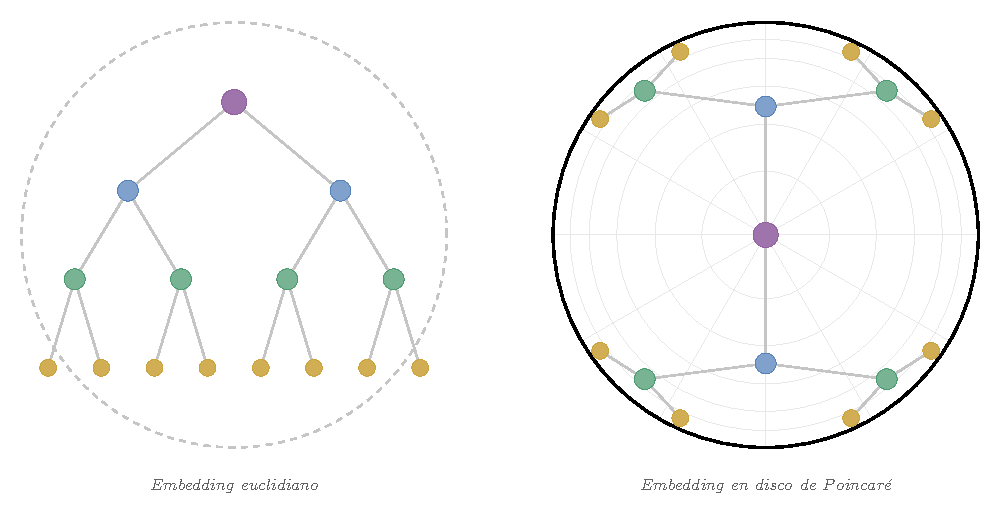
\includegraphics[width=0.9\textwidth]{images/hyperbolic_embedding.pdf}
    \caption{Comparison between Euclidean embedding (left) and embedding in the Poincaré disk (right) of a hierarchical tree. In $\mathbb{R}^2$, the leaves of the tree are compressed and the distances are distorted. In the Poincaré disk $\mathbb{D}^2$, the exponential growth of hyperbolic volume allows separating the branches with minimal distortion (\autoref{thm:embedding_arboles_hiperbolico}), whereas in $\mathbb{R}^d$ one needs $d = \Omega(\log n)$ (\autoref{prop:cota_inferior_euclidiano}).}
    \label{fig:hyperbolic_embedding_attention}
\end{figure}

\subsubsection{Hyperbolic Attention Networks}

The HANs of \citet{gulcehre2018hyperbolic} re-express attention in terms of hyperbolic operations, preserving the geometric properties of the space.

\begin{definition}[Hyperbolic Distance]\label{def:distancia_hiperbolica}
In the hyperboloid model, the hyperbolic distance between two points $\mathbf{x}, \mathbf{y} \in \mathbb{H}^n$ is defined as:

\begin{equation}
    d_{\mathbb{H}}(\mathbf{x}, \mathbf{y}) = \text{arccosh}(-\langle \mathbf{x}, \mathbf{y} \rangle_{\mathcal{L}})
    \label{eq:hyperbolic_distance}
\end{equation}

In the Poincaré model, the equivalent distance is:
\begin{equation}
d_{\mathbb{D}}(\mathbf{u}, \mathbf{v}) = \text{arccosh}\left(1 + 2\frac{\|\mathbf{u} - \mathbf{v}\|^2}{(1-\|\mathbf{u}\|^2)(1-\|\mathbf{v}\|^2)}\right)
\end{equation}
\end{definition}

\begin{theorem}[Properties of the Hyperbolic Distance]\label{thm:propiedades_distancia_hiperbolica}
The hyperbolic distance satisfies:
\begin{enumerate}
    \item \textbf{Metric}: $d_{\mathbb{H}}(\mathbf{x}, \mathbf{y}) \geq 0$ with equality if and only if $\mathbf{x} = \mathbf{y}$
    \item \textbf{Symmetry}: $d_{\mathbb{H}}(\mathbf{x}, \mathbf{y}) = d_{\mathbb{H}}(\mathbf{y}, \mathbf{x})$
    \item \textbf{Triangle inequality}: $d_{\mathbb{H}}(\mathbf{x}, \mathbf{z}) \leq d_{\mathbb{H}}(\mathbf{x}, \mathbf{y}) + d_{\mathbb{H}}(\mathbf{y}, \mathbf{z})$
    \item \textbf{Isometric invariance}: $d_{\mathbb{H}}(g\mathbf{x}, g\mathbf{y}) = d_{\mathbb{H}}(\mathbf{x}, \mathbf{y})$ for $g \in SO^+(1,n)$
\end{enumerate}
\end{theorem}

\begin{proof}
Properties (1)-(3) are verified directly from the distance formula. Positivity and equality result from the properties of arccosh. Symmetry is immediate from the symmetry of the Minkowski bilinear form $\langle \mathbf{x}, \mathbf{y} \rangle_M$. The triangle inequality is proven using the fact that arccosh is convex and that the geodesics of the hyperboloid are sections by planes passing through the origin. For (4), the isometries of the hyperboloid preserve the Minkowski form: $\langle g\mathbf{x}, g\mathbf{y} \rangle_M = \langle \mathbf{x}, \mathbf{y} \rangle_M$ for $g \in SO^+(1,n)$, and the distance depends only on $\langle \mathbf{x}, \mathbf{y} \rangle_M$.
\end{proof}

\begin{definition}[Generalized Hyperbolic Attention]\label{def:atencion_hiperbolica}
Hyperbolic attention is defined as:

\begin{equation}
    \text{HypAttn}(\mathbf{q}, \mathbf{K}, \mathbf{V}) = \text{softmax}(f(d_{\mathbb{H}}(\mathbf{q}, \mathbf{K}))) \odot_{\mathbb{H}} \mathbf{V}
    \label{eq:hyperbolic_attention}
\end{equation}

where:
\begin{itemize}
    \item $f: \mathbb{R} \to \mathbb{R}$ is an activation function (typically $f(x) = -\alpha x$ with $\alpha > 0$)
    \item $\odot_{\mathbb{H}}$ is the hyperbolic aggregation (generalization of the weighted sum)
    \item $\mathbf{q} \in \mathbb{H}^d$ is the hyperbolic query
    \item $\mathbf{K} = \{\mathbf{k}_i\}_{i=1}^n$ are the hyperbolic keys
    \item $\mathbf{V} = \{\mathbf{v}_i\}_{i=1}^n$ are the hyperbolic values
\end{itemize}
\end{definition}

\begin{definition}[Weighted Hyperbolic Aggregation]\label{def:agregacion_hiperbolica}
The hyperbolic aggregation of values $\{\mathbf{v}_i\}$ with weights $\{w_i\}$ is defined as:

\textbf{Einstein midpoint} (natural generalization in the Klein model):
\begin{equation}
\bigoplus_{i=1}^n w_i \mathbf{v}_i = \frac{\sum_{i=1}^n w_i \gamma(\mathbf{v}_i) \mathbf{v}_i}{\sum_{i=1}^n w_i \gamma(\mathbf{v}_i)}
\end{equation}
where $\gamma(\mathbf{v}) = \frac{1}{\sqrt{1-\|\mathbf{v}\|^2}}$ is the Lorentz factor and the denominator is a scalar sum (not a vector norm).

\textbf{Fréchet mean} (minimizer of geometric variance):
\begin{equation}
\bigoplus_{i=1}^n w_i \mathbf{v}_i = \arg\min_{\mathbf{x} \in \mathbb{H}^d} \sum_{i=1}^n w_i d_{\mathbb{H}}^2(\mathbf{x}, \mathbf{v}_i)
\end{equation}
\end{definition}

\textbf{Algorithm to compute the Fréchet mean}:

\begin{algorithm}[H]
\caption{Hyperbolic Fréchet Mean}
\begin{algorithmic}[1]
    \State \textbf{Input:} Points $\{\mathbf{v}_i\}_{i=1}^n \subset \mathbb{H}^d$, weights $\{w_i\}_{i=1}^n$
    \State Initialize $\mathbf{m}^{(0)} = \mathbf{v}_1$
    \For{$t = 0, 1, 2, \ldots$ until convergence}
        \State $\mathbf{g}^{(t)} = \sum_{i=1}^n w_i \log_{\mathbf{m}^{(t)}}^{\mathbb{H}}(\mathbf{v}_i)$
        \State $\mathbf{m}^{(t+1)} = \exp_{\mathbf{m}^{(t)}}^{\mathbb{H}}(\eta \mathbf{g}^{(t)})$
    \EndFor
    \State \textbf{Output:} $\mathbf{m}^{(\infty)}$
\end{algorithmic}
\end{algorithm}

\textbf{Theoretical properties of hyperbolic attention}:

\begin{proposition}[Equivariance under Isometries]\label{prop:equivarianza_atencion_hiperbolica}
For any isometry $g \in SO^+(1,n)$ of the hyperbolic space, if the hyperbolic aggregation $\odot_{\mathbb{H}}$ is equivariant under isometries (such as the Fréchet mean):
\begin{equation}
\text{HypAttn}(g\mathbf{q}, g\mathbf{K}, g\mathbf{V}) = g \cdot \text{HypAttn}(\mathbf{q}, \mathbf{K}, \mathbf{V})
\end{equation}
\end{proposition}

\begin{proof}[Proof idea]
The attention weights depend on hyperbolic distances: $\alpha_{ij} \propto \exp(f(d_{\mathbb{H}}(\mathbf{q}, \mathbf{k}_j)))$. Since $g$ is an isometry, $d_{\mathbb{H}}(g\mathbf{q}, g\mathbf{k}_j) = d_{\mathbb{H}}(\mathbf{q}, \mathbf{k}_j)$ (\autoref{thm:propiedades_distancia_hiperbolica}, property 4), so the attention weights are invariant: $\alpha_{ij}(g\mathbf{q}, g\mathbf{K}) = \alpha_{ij}(\mathbf{q}, \mathbf{K})$. For the Fréchet mean, equivariance follows from the fact that isometries preserve the objective function $\sum_i w_i d_{\mathbb{H}}^2(g\mathbf{x}, g\mathbf{v}_i) = \sum_i w_i d_{\mathbb{H}}^2(\mathbf{x}, \mathbf{v}_i)$, so $g$ maps the minimizer to $g$ of the minimizer.
\end{proof}

\begin{corollary}[Similarity Invariance]\label{cor:invarianza_similaridad}
Hyperbolic attention is invariant under transformations that preserve the hierarchical relations in the data.
\end{corollary}

\begin{proof}
The transformations that preserve hierarchical relations are precisely the isometries of hyperbolic space, that is, the group $SO^+(1,n)$: these preserve the hyperbolic distance $d_{\mathbb{H}}$ and, with it, the proximity relations that encode the hierarchy. By \autoref{prop:equivarianza_atencion_hiperbolica}, hyperbolic attention is equivariant under every isometry $g \in SO^+(1,n)$. In particular, the attention weights $\alpha_{ij} \propto \exp(-d_{\mathbb{H}}(\mathbf{q}_i, \mathbf{k}_j))$ are invariant under isometries (since $d_{\mathbb{H}}(g\mathbf{q}_i, g\mathbf{k}_j) = d_{\mathbb{H}}(\mathbf{q}_i, \mathbf{k}_j)$), which implies that the similarities computed by the attention mechanism are invariant under transformations that preserve the hierarchical structure.
\end{proof}

\textbf{Specific computational advantages}:

\begin{itemize}
    \item \textbf{Compact representation}: Complex hierarchies require smaller dimensions than Euclidean embeddings
    \item \textbf{Implicit regularization}: Hyperbolic geometry prevents overfitting on hierarchical data
    \item \textbf{Interpretability}: The hyperbolic distance directly reflects hierarchical relations
    \item \textbf{Scalability}: Efficient operations in the Poincaré model
\end{itemize}

\subsubsection{Hyperbolic Vision \gls{Transformer}}

The Hyperbolic Vision Transformer (HVT) of \citet{hvt2024hyperbolic} represents a fundamental extension of the \gls{ViT} architecture that integrates hyperbolic geometry to efficiently capture hierarchical structures in visual data.

\textbf{Fundamental architecture of HVT}:

The HVT architecture consists of three main components that operate in hyperbolic space:

\begin{definition}[Hyperbolic Projections in HVT]\label{def:hvt_projections}
The query, key, value projections in HVT are reformulated through exponential/logarithmic maps:

\begin{align}
    \mathbf{Q} &= \text{exp}_{\mathbf{0}}^{\mathbb{H}}(\mathbf{W}_Q \text{log}_{\mathbf{0}}^{\mathbb{H}}(\mathbf{X})) \\
    \mathbf{K} &= \text{exp}_{\mathbf{0}}^{\mathbb{H}}(\mathbf{W}_K \text{log}_{\mathbf{0}}^{\mathbb{H}}(\mathbf{X})) \\
    \mathbf{V} &= \text{exp}_{\mathbf{0}}^{\mathbb{H}}(\mathbf{W}_V \text{log}_{\mathbf{0}}^{\mathbb{H}}(\mathbf{X}))
    \label{eq:hyperbolic_projections}
\end{align}

where $\text{exp}_{\mathbf{0}}^{\mathbb{H}}: T_{\mathbf{0}}\mathbb{H}^d \to \mathbb{H}^d$ and $\text{log}_{\mathbf{0}}^{\mathbb{H}}: \mathbb{H}^d \to T_{\mathbf{0}}\mathbb{H}^d$ are the hyperbolic exponential and logarithmic maps at the origin.
\end{definition}

\textbf{Geometric justification.}\label{rem:hvt_geometry} The map $\text{log}_{\mathbf{0}}^{\mathbb{H}}$ projects hyperbolic representations to the Euclidean tangent space at the origin, where standard linear transformations $\mathbf{W}_Q, \mathbf{W}_K, \mathbf{W}_V$ are applied. The map $\text{exp}_{\mathbf{0}}^{\mathbb{H}}$ subsequently projects the result back to hyperbolic space, preserving geometric properties.

\textbf{Complete formulation of the hyperbolic attention mechanism}:

\begin{definition}[Hyperbolic Multi-Head Attention]\label{def:hvt_multihead}
The multi-head attention mechanism in HVT is defined as:

\begin{equation}
\text{HypMultiHead}(\mathbf{X}) = \text{exp}_{\mathbf{0}}^{\mathbb{H}}\left(\mathbf{W}_O \text{Concat}(\text{head}_1, \ldots, \text{head}_h)\right)
\label{eq:hvt_multihead}
\end{equation}

where each head $\text{head}_i$ operates in hyperbolic space:

\begin{equation}
\text{head}_i = \text{softmax}\left(-\alpha d_{\mathbb{H}}(\mathbf{Q}_i, \mathbf{K}_i)\right) \odot_{\mathbb{H}} \mathbf{V}_i
\label{eq:hvt_head}
\end{equation}

with $\alpha > 0$ a scale parameter and $\odot_{\mathbb{H}}$ the hyperbolic aggregation (Fréchet mean).
\end{definition}

\textbf{Training procedures and numerical stability}:

Training HVT requires special considerations to maintain numerical stability in hyperbolic space:

\begin{enumerate}
    \item \textbf{Hyperbolic initialization}: The parameters are initialized through exponential projection of small Gaussian distributions:
    \begin{equation}
    \mathbf{w}^{(0)} = \text{exp}_{\mathbf{0}}^{\mathbb{H}}(\epsilon \mathbf{z}), \quad \mathbf{z} \sim \mathcal{N}(0, \mathbf{I}), \quad \epsilon \ll 1
    \end{equation}

    \item \textbf{Projection to the Poincaré ball}: To maintain numerical stability, all points are projected to $\|\mathbf{x}\| < 1 - \delta$ with $\delta = 10^{-5}$:
    \begin{equation}
    \text{proj}(\mathbf{x}) = \begin{cases}
    \mathbf{x} & \text{if } \|\mathbf{x}\| \leq 1 - \delta \\
    \frac{(1-\delta)\mathbf{x}}{\|\mathbf{x}\|} & \text{otherwise}
    \end{cases}
    \end{equation}

    \item \textbf{Riemannian Optimization}: The RSGD optimizer (Riemannian Stochastic Gradient Descent) is used:
    \begin{equation}
    \mathbf{x}^{(t+1)} = \text{exp}_{\mathbf{x}^{(t)}}^{\mathbb{H}}\left(-\eta \text{grad}^{\mathbb{H}} L(\mathbf{x}^{(t)})\right)
    \end{equation}
    where $\text{grad}^{\mathbb{H}} L = \lambda_{\mathbf{x}}^{-2} \nabla L$ is the Riemannian gradient with $\lambda_{\mathbf{x}} = \frac{2}{1-\|\mathbf{x}\|^2}$.
\end{enumerate}

\begin{theorem}[Convergence of RSGD on Manifolds]\label{thm:hvt_convergence}
Let $L: \mathbb{H}^d \to \mathbb{R}$ be a geodesically convex function with $M$-Lipschitz Riemannian gradient. The RSGD algorithm with learning rate $\eta < 1/M$ satisfies, for the averaged iterate $\bar{\mathbf{x}}^{(T)} = \frac{1}{T}\sum_{t=0}^{T-1} \mathbf{x}^{(t)}$ (average in the tangent space):
\begin{equation}
\mathbb{E}[L(\bar{\mathbf{x}}^{(T)})] - L(\mathbf{x}^*) \leq \frac{d_{\mathbb{H}}^2(\mathbf{x}^{(0)}, \mathbf{x}^*)}{2\eta T} + \frac{\eta M \sigma^2}{2}
\end{equation}
where $\sigma^2$ is the variance of the stochastic gradient and $\mathbf{x}^*$ is a global minimizer. This result is an adaptation of the convergence theorem of \citet{bonnabel2013stochastic} for stochastic gradient descent on Riemannian manifolds.
\end{theorem}

\textbf{Experimental results and ablation}:

The experiments of \citet{hvt2024hyperbolic} demonstrate significant advantages of HVT over standard \gls{ViT}:

\begin{itemize}
    \item \textbf{ImageNet-1K}: HVT-Base achieves 84.2\% top-1 accuracy with 30\% fewer parameters than ViT-Base
    \item \textbf{CIFAR-100}: Improvement of 2.8\% in accuracy with hyperbolic embeddings of dimension $d=256$ vs. Euclidean of $d=512$
    \item \textbf{Hierarchical data}: In biological species classification (taxonomic structure), HVT surpasses \gls{ViT} by 5.3\%
\end{itemize}

\subsubsection{HyPE-GT: Hyperbolic Positional Encodings}

HyPE-GT (Hyperbolic Positional Encodings for Graph Transformers) of \citet{hypegt2023} introduces learnable positional encodings in hyperbolic space that naturally capture hierarchical structures in graphs.

\textbf{Mathematical formulation of HyPE}:

\begin{definition}[Hyperbolic Positional Encodings]\label{def:hype_encoding}
For a graph $\mathcal{G} = (V, E)$, the hyperbolic positional encodings are defined as:

\begin{equation}
    \mathbf{PE}_i^{\mathbb{H}} = \text{HypMLP}(\mathbf{h}_i^{(0)}, \mathbf{s}_i)
    \label{eq:hyperbolic_positional_encoding}
\end{equation}

where:
\begin{itemize}
    \item $\mathbf{h}_i^{(0)} \in \mathbb{R}^{d_0}$ are the initial features of node $i$
    \item $\mathbf{s}_i \in \mathbb{R}^{d_s}$ is the structural vector that encodes topological properties of the node
    \item $\text{HypMLP}: \mathbb{R}^{d_0 + d_s} \to \mathbb{H}^d$ is a multilayer neural network with hyperbolic output
\end{itemize}
\end{definition}

\begin{definition}[Node Structural Vector]\label{def:structural_vector}
The structural vector $\mathbf{s}_i$ captures local and global topological properties:

\begin{equation}
\mathbf{s}_i = [\text{deg}(i), \text{CC}(i), \text{BC}(i), \text{PR}(i), \mathbf{d}_i^{\text{ecc}}]
\end{equation}

where:
\begin{itemize}
    \item $\text{deg}(i)$ is the degree of the node
    \item $\text{CC}(i)$ is the clustering coefficient
    \item $\text{BC}(i)$ is the betweenness centrality
    \item $\text{PR}(i)$ is the PageRank
    \item $\mathbf{d}_i^{\text{ecc}} \in \mathbb{R}^k$ is the vector of eccentricities (distances to representative nodes)
\end{itemize}
\end{definition}

The HyPE encodings are integrated into the \gls{Transformer} architecture through hyperbolic combination with the Möbius operations, and attention is computed over the combined embeddings.

\begin{remark}[Dimensional advantage of hyperbolic embeddings]\label{rem:hypegt_expressiveness}
The hyperbolic positional encodings of HyPE-GT \citep{hypegt2023} benefit from the general property that hyperbolic embeddings require smaller dimensions than Euclidean ones to represent hierarchical structures. By \autoref{thm:embedding_arboles_hiperbolico}, a tree with $n$ vertices can be embedded in $\mathbb{H}^2$ with distortion $(1+\varepsilon)$, whereas Euclidean embeddings with bounded distortion require dimension $d = \Omega(\log n)$ (\autoref{prop:cota_inferior_euclidiano}). This theoretical advantage motivates the use of hyperbolic encodings in HyPE-GT, although \citet{hypegt2023} do not formally establish expressiveness bounds for their architecture, their contribution being mainly empirical.
\end{remark}

\subsection{Attention and Embeddings on the Sphere}\label{subsec:atencion_esfera}

While the previous section explores attention in spaces of negative curvature, the unit sphere $S^{d-1}$ constitutes the most relevant space of constant positive curvature for attention mechanisms. Normalizing embeddings to $S^{d-1}$ induces a direct connection between the dot product (the basis of standard attention) and the spherical geodesic distance.

\begin{proposition}[Dot Product--Cosine Similarity Equivalence on $S^{d-1}$]\label{prop:dot_product_sphere}
Let $\hat{\mathbf{q}}, \hat{\mathbf{k}} \in S^{d-1}$ be normalized embeddings, that is, $\hat{\mathbf{q}} = \mathbf{q}/\|\mathbf{q}\|$ and $\hat{\mathbf{k}} = \mathbf{k}/\|\mathbf{k}\|$. Then:
\begin{equation}
\hat{\mathbf{q}}^T \hat{\mathbf{k}} = \cos\bigl(d_{S^{d-1}}(\hat{\mathbf{q}}, \hat{\mathbf{k}})\bigr)
\label{eq:dot_geodesic_sphere}
\end{equation}
where $d_{S^{d-1}}(\hat{\mathbf{q}}, \hat{\mathbf{k}}) = \arccos(\hat{\mathbf{q}}^T \hat{\mathbf{k}})$ is the geodesic distance on $S^{d-1}$. Consequently, scaled attention over normalized embeddings
\[
\alpha_{ij} = \frac{\exp\bigl(\hat{\mathbf{q}}_i^T \hat{\mathbf{k}}_j / \tau\bigr)}{\sum_l \exp\bigl(\hat{\mathbf{q}}_i^T \hat{\mathbf{k}}_l / \tau\bigr)}
\]
operates exclusively with spherical geodesic distances (cf.\ \autoref{def:dot_product_similarity}).
\end{proposition}

\begin{proof}
By definition of the metric on $S^{d-1}$ (see \autoref{def:esfera_n}), the geodesic distance between $\hat{\mathbf{q}}, \hat{\mathbf{k}} \in S^{d-1}$ is $d_{S^{d-1}}(\hat{\mathbf{q}}, \hat{\mathbf{k}}) = \arccos(\hat{\mathbf{q}}^T \hat{\mathbf{k}})$. Applying the cosine to both sides directly yields identity~\eqref{eq:dot_geodesic_sphere}. Since $\|\hat{\mathbf{q}}\| = \|\hat{\mathbf{k}}\| = 1$, the dot product $\hat{\mathbf{q}}^T \hat{\mathbf{k}}$ does not depend on magnitudes, but only on the geodesic angle, and the attention weights $\alpha_{ij}$ are a monotonically decreasing function of the geodesic distance $d_{S^{d-1}}$.
\end{proof}

\autoref{prop:dot_product_sphere} motivates the use of normalized embeddings in classification tasks: by eliminating the magnitude, the decision boundary depends exclusively on angles.

\begin{definition}[Angular Classifier]\label{def:clasificador_angular}
Let $\hat{\mathbf{f}}(\mathbf{x}) = \mathbf{f}(\mathbf{x})/\|\mathbf{f}(\mathbf{x})\| \in S^{d-1}$ be the normalized embedding of an input $\mathbf{x}$, and let $\hat{\mathbf{w}}_c = \mathbf{w}_c/\|\mathbf{w}_c\| \in S^{d-1}$ be the normalized weights for each class $c \in \{1, \ldots, C\}$. An \textit{angular classifier} \citep{wang2017normface} produces logits of the form:
\begin{equation}
z_c(\mathbf{x}) = s \cdot \hat{\mathbf{f}}(\mathbf{x})^T \hat{\mathbf{w}}_c = s \cos\theta_c
\label{eq:clasificador_angular}
\end{equation}
where $\theta_c = d_{S^{d-1}}(\hat{\mathbf{f}}(\mathbf{x}), \hat{\mathbf{w}}_c) \in [0, \pi]$ is the geodesic distance to the prototype of class $c$, and $s > 0$ is a scale parameter needed to control the concentration of the softmax distribution (without $s$, the logits would be bounded in $[-1, 1]$, producing excessively uniform probability distributions).
\end{definition}

\begin{definition}[Generalized Angular Margin Loss]\label{def:perdida_margen_angular}
Given the angular classifier structure (\autoref{def:clasificador_angular}), an \textit{angular margin loss} modifies the logit of the correct class $y$ through a margin function $g: [0, \pi] \to \mathbb{R}$:
\begin{equation}
\mathcal{L} = -\log \frac{\exp\bigl(s \cdot g(\theta_y)\bigr)}{\exp\bigl(s \cdot g(\theta_y)\bigr) + \sum_{c \neq y} \exp\bigl(s \cos\theta_c\bigr)}
\label{eq:perdida_margen_angular}
\end{equation}
The main instances of this family are:
\begin{enumerate}
    \item \textbf{NormFace} \citep{wang2017normface}: $g(\theta) = \cos\theta$ (no margin, normalized baseline).
    \item \textbf{SphereFace} \citep{liu2017sphereface}: $g(\theta) = \cos(m\theta)$ with $m \in \mathbb{N}$, $m \geq 2$ (multiplicative angular margin).
    \item \textbf{CosFace} \citep{wang2018cosface}: $g(\theta) = \cos\theta - m$ with $m > 0$ (additive margin in cosine space).
    \item \textbf{ArcFace} \citep{deng2019arcface}: $g(\theta) = \cos(\theta + m)$ with $m > 0$ (additive angular margin).
\end{enumerate}
\end{definition}

\begin{proposition}[Geodesic Interpretation of the Angular Margin]\label{prop:interpretacion_geodesica_margen}
In ArcFace, the margin $m > 0$ imposes a geodesic separation of exactly $m$ radians on $S^{d-1}$ between the embedding and the nearest decision boundary.
\end{proposition}

\begin{proof}
Without a margin, the decision boundary between classes $y$ and $c$ lies where $\cos\theta_y = \cos\theta_c$, that is, where the geodesic distances to both prototypes coincide. With ArcFace, the condition for correct classification requires $\cos(\theta_y + m) \geq \cos\theta_c$, which is equivalent to $\theta_y + m \leq \theta_c$ (in the range $[0, \pi]$ where the cosine is monotonically decreasing). At the boundary, $\theta_y + m = \theta_c$, and therefore the embedding must be at geodesic distance at least $m$ radians closer to its class prototype than to any other. Since $\theta_y = d_{S^{d-1}}(\hat{\mathbf{f}}(\mathbf{x}), \hat{\mathbf{w}}_y)$, this separation is intrinsically geodesic.
\end{proof}

\begin{remark}[Contrastive Learning as Attention on $S^{d-1}$]\label{rem:contrastive_sphere}
The InfoNCE loss used in multimodal models constitutes a particular case of angular classification. Given normalized embeddings $\hat{\mathbf{z}}_i^A, \hat{\mathbf{z}}_j^B \in S^{d-1}$ from two modalities, the loss
\[
\mathcal{L}_{\text{InfoNCE}} = -\log \frac{\exp\bigl(\hat{\mathbf{z}}_i^{A\,T} \hat{\mathbf{z}}_i^B / \tau\bigr)}{\sum_{j} \exp\bigl(\hat{\mathbf{z}}_i^{A\,T} \hat{\mathbf{z}}_j^B / \tau\bigr)}
\]
is exactly an angular classifier with $s = 1/\tau$, $g(\theta) = \cos\theta$, and the classes defined dynamically by the batch. Thus, contrastive learning performs angular classification over the sphere, where the temperature $\tau$ controls the concentration of softmax attention over the nearest geodesic neighbors.
\end{remark}

\subsection{Parallel Transport and Connections}

Parallel transport provides a fundamental mechanism for comparing tangent vectors at different points of a Riemannian manifold, preserving the intrinsic geometric structure. This concept is essential for formulating attention mechanisms on non-Euclidean manifolds.

\subsubsection{Mathematical Foundations of Parallel Transport}

We recall that the \textit{Levi-Civita connection} $\nabla$ of a Riemannian manifold $(M, g)$ is the unique affine connection compatible with the metric and torsion-free (\autoref{def:conexion_levi_civita_gdl} of \autoref{ch:gdl}), determined in local coordinates by the Christoffel symbols $\Gamma^k_{ij}$.\label{def:levi_civita_attention}\label{eq:christoffel_symbols_attention}

The \textit{parallel transport} along a curve $\gamma: [0,1] \to M$ is given by the equation $\nabla_{\dot{\gamma}(t)} V(t) = 0$, which in local coordinates translates into $\frac{dV^k}{dt} + \Gamma^k_{ij} \frac{dx^i}{dt} V^j = 0$ (see \autoref{def:transporte_paralelo_formal} of \autoref{ch:gdl} for the general case in principal bundles).\label{def:parallel_transport_attention}\label{eq:parallel_transport}\label{eq:parallel_transport_coordinates}

\begin{theorem}[Existence and Uniqueness of Parallel Transport]\label{thm:existence_parallel_transport}
Given a smooth curve $\gamma: [0,1] \to M$ and an initial vector $v_0 \in T_{\gamma(0)}M$, there exists a unique parallel vector field $V(t)$ along $\gamma$ with $V(0) = v_0$.

Parallel transport defines a linear isometry:
\begin{equation}
\Gamma_\gamma: T_{\gamma(0)}M \to T_{\gamma(1)}M
\end{equation}
that satisfies $\Gamma_\gamma(v_0) = V(1)$.
\end{theorem}

\begin{proof}
Equation~\eqref{eq:parallel_transport_coordinates} is a linear system of first-order ODEs. By the Picard-Lindelöf theorem, given an initial value $V(0) = v_0$, there exists a unique solution $V(t)$ defined for $t \in [0,1]$.

The metric preservation follows from the compatibility of $\nabla$ with $g$:
\begin{align}
\frac{d}{dt}\langle V(t), W(t) \rangle &= \langle \nabla_{\dot{\gamma}} V, W \rangle + \langle V, \nabla_{\dot{\gamma}} W \rangle \\
&= 0 \quad \text{(if $V$ and $W$ are parallel)}
\end{align}

Therefore, $\langle \Gamma_\gamma(v), \Gamma_\gamma(w) \rangle_{\gamma(1)} = \langle v, w \rangle_{\gamma(0)}$ for all $v, w \in T_{\gamma(0)}M$.
\end{proof}

\begin{proposition}[Properties of Parallel Transport]\label{prop:parallel_transport_properties}
Parallel transport $\Gamma_\gamma: T_{\gamma(0)}M \to T_{\gamma(1)}M$ satisfies:

\begin{enumerate}
    \item \textbf{Linearity}: $\Gamma_\gamma(\alpha u + \beta v) = \alpha \Gamma_\gamma(u) + \beta \Gamma_\gamma(v)$
    \item \textbf{Metric preservation}: $g_{\gamma(1)}(\Gamma_\gamma(u), \Gamma_\gamma(v)) = g_{\gamma(0)}(u, v)$
    \item \textbf{Concatenation property}: For paths $\gamma_1, \gamma_2$ with $\gamma_1(1) = \gamma_2(0)$:
    \begin{equation}
    \Gamma_{\gamma_2 * \gamma_1} = \Gamma_{\gamma_2} \circ \Gamma_{\gamma_1}
    \end{equation}
    \item \textbf{Inversion}: $\Gamma_{\gamma^{-1}} = (\Gamma_\gamma)^{-1}$ where $\gamma^{-1}(t) = \gamma(1-t)$
\end{enumerate}
\end{proposition}

\begin{proof}
\textbf{(1) Linearity}: Since parallel transport is defined as the solution of the equation $\nabla_{\dot{\gamma}} V = 0$, which is linear in $V$, the uniqueness of solutions of linear ODEs guarantees the linearity of the operator $\Gamma_\gamma$.

\textbf{(2) Metric preservation}: If $\nabla$ is the Levi-Civita connection, compatible with the metric, then for parallel fields $V, W$ along $\gamma$:
\[
\frac{d}{dt} g(V, W) = g(\nabla_{\dot{\gamma}} V, W) + g(V, \nabla_{\dot{\gamma}} W) = 0
\]
so $g(V,W)$ is constant along $\gamma$.

\textbf{(3) Concatenation}: Let $V$ be a parallel field along $\gamma_1$ with $V(0) = v$. Then $V(1) = \Gamma_{\gamma_1}(v)$. Let $W$ be parallel along $\gamma_2$ with $W(0) = V(1)$. Then $W(1) = \Gamma_{\gamma_2}(\Gamma_{\gamma_1}(v))$. But the concatenation $\gamma_2 * \gamma_1$ with field $V$ followed by $W$ is parallel along the complete path.

\textbf{(4) Inversion}: If $V$ is parallel along $\gamma$, then $V(\gamma^{-1}(t)) = V(\gamma(1-t))$ is parallel along $\gamma^{-1}$, so $\Gamma_{\gamma^{-1}} \circ \Gamma_\gamma = \text{Id}$.
\end{proof}

\begin{figure}[ht]
    \centering
    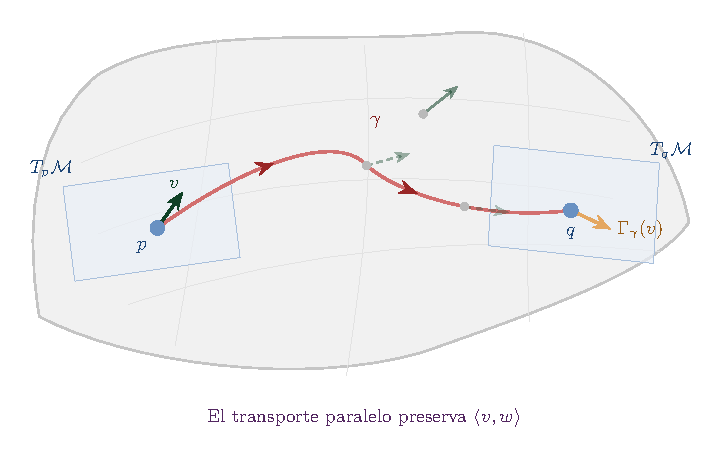
\includegraphics[width=0.8\textwidth]{images/parallel_transport_surface.pdf}
    \caption{Parallel transport of a tangent vector along a curve $\gamma$ on a surface. The vector $V(t)$ satisfies $\nabla_{\dot{\gamma}} V = 0$, keeping its norm and relative angle to the curve constant. The dependence of the result on the chosen path (holonomy) reflects the curvature of the surface and motivates attention with parallel transport (\autoref{def:attention_parallel_transport}).}
    \label{fig:parallel_transport_attention}
\end{figure}

\subsubsection{Algorithm to Compute Geodesics and Parallel Transport}

In practice, parallel transport is computed numerically through integration of equation~\eqref{eq:parallel_transport_coordinates} along geodesics.

We recall that a \textit{geodesic} is a curve $\gamma$ that satisfies $\nabla_{\dot{\gamma}} \dot{\gamma} = 0$, or equivalently in local coordinates $\ddot{x}^k + \Gamma^k_{ij} \dot{x}^i \dot{x}^j = 0$ (\autoref{def:geodesica} of \autoref{ch:gdl}).\label{def:geodesic_attention}\label{eq:geodesic_equation}

\begin{algorithm}[H]
\caption{Computation of Parallel Transport on Riemannian Manifolds}
\label{alg:parallel_transport_computation}
\begin{algorithmic}[1]
    \State \textbf{Input:} Initial point $p \in M$, final point $q \in M$, vector $v \in T_p M$
    \State \textbf{Output:} Transported vector $\Gamma_{pq}(v) \in T_q M$
    \State
    \State \textbf{Step 1: Compute geodesic} $\gamma: [0,1] \to M$ with $\gamma(0) = p$, $\gamma(1) = q$
    \State Solve the geodesic equation~\eqref{eq:geodesic_equation} using fourth-order Runge-Kutta
    \State
    \State \textbf{Step 2: Initialize} parallel vector field $V(0) = v$
    \State
    \State \textbf{Step 3: Integrate} parallel transport equation~\eqref{eq:parallel_transport_coordinates}
    \For{$t = 0$ to $1$ (discretization $\Delta t = 1/N$)}
        \State Compute Christoffel symbols $\Gamma^k_{ij}(\gamma(t))$ at the current point
        \State Update $V(t + \Delta t)$ using the Runge-Kutta method:
        \State $\quad V^k(t + \Delta t) = V^k(t) - \Delta t \cdot \Gamma^k_{ij}(\gamma(t)) \dot{\gamma}^i(t) V^j(t)$
    \EndFor
    \State
    \State \textbf{Return} $\Gamma_{pq}(v) = V(1)$
\end{algorithmic}
\end{algorithm}

\subsubsection{Worked Example: Parallel Transport on the Sphere $S^2$}

We develop a complete example of parallel transport on the unit sphere, where the formulas admit closed-form expressions.

\begin{example}[Parallel Transport on $S^2$]\label{ex:parallel_transport_sphere}
Consider the unit sphere $S^2 = \{\mathbf{x} \in \mathbb{R}^3 : \|\mathbf{x}\| = 1\}$ with the metric induced from Euclidean space.

\textbf{Geodesics on $S^2$}: The geodesics are great circles. For two non-antipodal points $p, q \in S^2$, the geodesic is given by:
\begin{equation}
\gamma(t) = \frac{\sin((1-t)\theta)}{\sin\theta} p + \frac{\sin(t\theta)}{\sin\theta} q, \quad t \in [0,1]
\end{equation}
where $\theta = \arccos(\langle p, q \rangle)$ is the angle between $p$ and $q$.

\textbf{Explicit formula for parallel transport}: For a tangent vector $v \in T_p S^2$ (with $\langle v, p \rangle = 0$), the parallel transport to $T_q S^2$ along the geodesic $\gamma$ is:

\begin{equation}
\Gamma_{\gamma_{pq}}(v) = v - \frac{\langle v, q \rangle + \langle v, p \rangle}{1 + \langle p, q \rangle}(p + q)
\label{eq:parallel_transport_sphere_formula}
\end{equation}

Taking advantage of the fact that $v \perp p$ (that is, $\langle v, p \rangle = 0$), this formula simplifies to:
\begin{equation}
\Gamma_{\gamma_{pq}}(v) = v - \frac{\langle v, q \rangle}{1 + \langle p, q \rangle}(p + q)
\end{equation}

\textbf{Verification of properties}:
\begin{enumerate}
    \item \textbf{Tangency}: $\langle \Gamma_{\gamma_{pq}}(v), q \rangle = 0$ (the transported vector is tangent at $q$)
    \item \textbf{Norm preservation}: $\|\Gamma_{\gamma_{pq}}(v)\| = \|v\|$
    \item \textbf{Angle preservation}: For $v, w \in T_p S^2$:
    \begin{equation}
    \langle \Gamma_{\gamma_{pq}}(v), \Gamma_{\gamma_{pq}}(w) \rangle = \langle v, w \rangle
    \end{equation}
\end{enumerate}
\end{example}

\subsubsection{Parallel Transport in Attention Mechanisms}

Parallel transport allows formulating geometrically consistent attention mechanisms on Riemannian manifolds.

\begin{definition}[Attention with Parallel Transport]\label{def:attention_parallel_transport}
Let $M$ be a Riemannian manifold and $\{x_i\}_{i=1}^n \subset M$ a set of points (tokens) on the manifold. For features $\{f_i \in T_{x_i}M\}_{i=1}^n$, attention with parallel transport at point $x_j$ is defined as:

\begin{equation}
\text{Attn}_{\text{PT}}(x_j, \{x_i, f_i\}) = \sum_{i=1}^n \alpha_{ij} \Gamma_{\gamma_{ij}}(f_i)
\label{eq:attention_parallel_transport}
\end{equation}

where:
\begin{itemize}
    \item $\gamma_{ij}$ is the geodesic from $x_i$ to $x_j$
    \item $\Gamma_{\gamma_{ij}}: T_{x_i}M \to T_{x_j}M$ is the parallel transport
    \item $\alpha_{ij} = \text{softmax}_i(-d_M(x_i, x_j)^2)$ are the attention weights based on geodesic distance
\end{itemize}
\end{definition}

\begin{theorem}[Equivariance under Isometries]\label{thm:attention_parallel_transport_equivariance}
Let $\phi: M \to M$ be an isometry of the Riemannian manifold. Attention with parallel transport satisfies:

\begin{equation}
\text{Attn}_{\text{PT}}(\phi(x_j), \{\phi(x_i), d\phi_{x_i}(f_i)\}) = d\phi_{x_j}(\text{Attn}_{\text{PT}}(x_j, \{x_i, f_i\}))
\end{equation}

where $d\phi_x: T_x M \to T_{\phi(x)}M$ is the differential of $\phi$.
\end{theorem}

\begin{proof}
Isometries preserve geodesics and parallel transport:
\begin{enumerate}
    \item $\phi(\gamma_{ij}(t)) = \gamma_{\phi(i)\phi(j)}(t)$ (geodesics map to geodesics)
    \item $d\phi \circ \Gamma_{\gamma_{ij}} = \Gamma_{\phi(\gamma_{ij})} \circ d\phi$ (commutativity with transport)
    \item $d_M(\phi(x_i), \phi(x_j)) = d_M(x_i, x_j)$ (distance preservation)
\end{enumerate}

Applying these properties:
\begin{align}
\text{Attn}_{\text{PT}}(\phi(x_j), \{\phi(x_i), d\phi(f_i)\}) &= \sum_i \alpha_{ij} \Gamma_{\gamma_{\phi(i)\phi(j)}}(d\phi(f_i)) \\
&= \sum_i \alpha_{ij} d\phi(\Gamma_{\gamma_{ij}}(f_i)) \\
&= d\phi\left(\sum_i \alpha_{ij} \Gamma_{\gamma_{ij}}(f_i)\right) \\
&= d\phi(\text{Attn}_{\text{PT}}(x_j, \{x_i, f_i\})) \qquad \square
\end{align}
\end{proof}

\subsubsection{Applications in Geometric Deep Learning}

Parallel transport has found successful applications in attention architectures for non-Euclidean data:

\begin{itemize}
    \item \textbf{Climate models on the sphere}: Attention on meteorological data defined on $S^2$ using parallel transport to aggregate information from different locations while preserving orientations

    \item \textbf{3D mesh processing}: Convolutions on surfaces where parallel transport allows comparing tangent features at different vertices of the mesh

    \item \textbf{Neural networks in shape spaces}: Analysis of anatomical shapes represented as points on Riemannian manifolds (e.g., Stiefel manifold, Grassmannian)

    \item \textbf{Hyperbolic attention with transport}: Combination of hyperbolic geometry (for hierarchies) with parallel transport (for geometrically consistent aggregation)
\end{itemize}

\begin{example}[Practical implementation: Attention on $SO(3)$]\label{ex:attention_so3}
For orientation data represented as rotations $R_i \in SO(3)$, attention with parallel transport allows aggregating information while respecting the Lie geometry of the group.

Given a set of orientations $\{R_i\}$ with features $\{f_i \in T_{R_i}SO(3) \cong \mathfrak{so}(3)\}$:

\begin{enumerate}
    \item \textbf{Compute geodesics}: For $R_i, R_j \in SO(3)$, the geodesic is:
    \begin{equation}
    \gamma(t) = R_i \exp(t \log(R_i^{-1} R_j)), \quad t \in [0,1]
    \end{equation}

    \item \textbf{Parallel transport}: In Lie groups, parallel transport through left translation:
    \begin{equation}
    \Gamma_{\gamma_{ij}}(f_i) = \text{Ad}_{R_i^{-1}R_j}(f_i)
    \end{equation}
    where $\text{Ad}_R: \mathfrak{so}(3) \to \mathfrak{so}(3)$ is the adjoint representation.

    \item \textbf{Aggregation}: Compute weights $\alpha_{ij} \propto \exp(-\|R_i^{-1}R_j\|_F^2)$ and aggregate:
    \begin{equation}
    \text{Attn}(R_j) = \sum_i \alpha_{ij} \text{Ad}_{R_i^{-1}R_j}(f_i)
    \end{equation}
\end{enumerate}

This formulation is invariant under global rotations and preserves the group structure of $SO(3)$.
\end{example}
